\chapter{Perancangan}
\label{chap:perancangan}

\section{Perancangan Kelas Akibat Kurikulum 2018}

Pada subbab ini akan menjelaskan perancangan kelas akibat kurikulum 2018 dari hasil analisis pada subbab \ref{subbab:analisissiamodels} \& \ref{subbab:analisisifstudentportal}. Diagram kelas akibat kurikulum 2018 dibagi menjadi beberapa bagian yang dapat dilihat pada gambar \ref{fig:siamodels_class_2018} untuk diagram kelas SIAModels yang berubah pada kelas \texttt{Nilai} dan untuk diagram kelas lengkapnya dapat dilihat pada gambar \ref{fig:2_siamodels_class}. Gambar \ref{fig:siamodels_class_2018_kurikulum_1}, \ref{fig:siamodels_class_2018_kurikulum_2}, \ref{fig:siamodels_class_2018_kurikulum_3}, \ref{fig:siamodels_class_2018_kurikulum_4}, dan \ref{fig:siamodels_class_2018_kurikulum_5} untuk diagram kelas yang merepresentasikan mata kuliah pada kurikulum 2018. Deskripsi kelas berserta fungsi dari diagram kelas tersebut adalah sebagai berikut:

\begin{figure}[H]
\centering
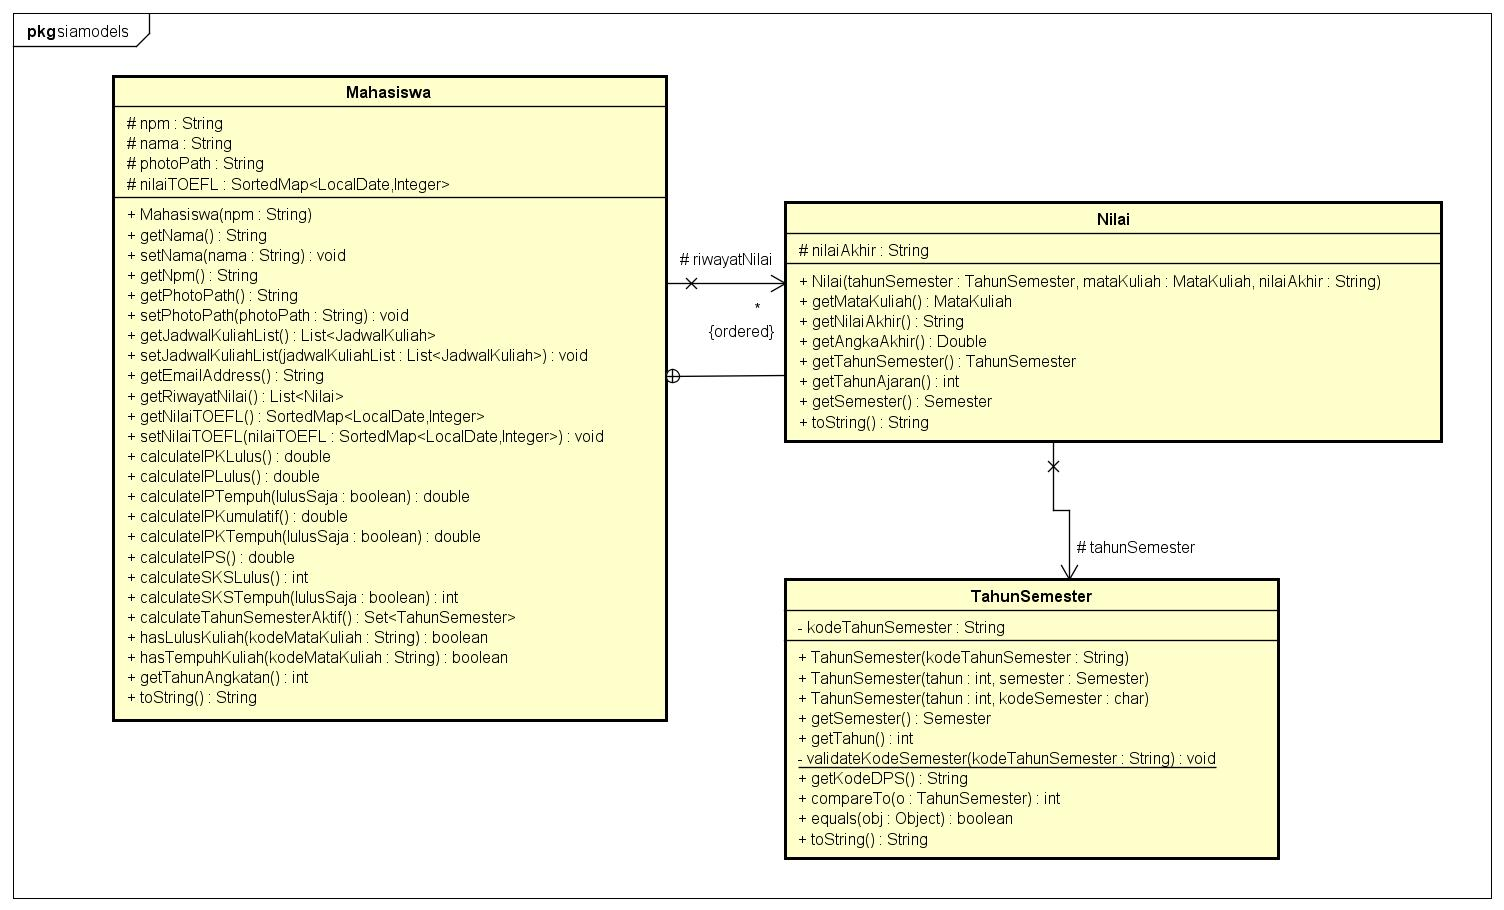
\includegraphics[scale=0.3]{Gambar/class-diagram-siamodels-new}
\caption{Diagram Kelas SIAModels Bagian \texttt{Nilai}}
\label{fig:siamodels_class_2018}
\end{figure}

\begin{figure}[H]
\centering
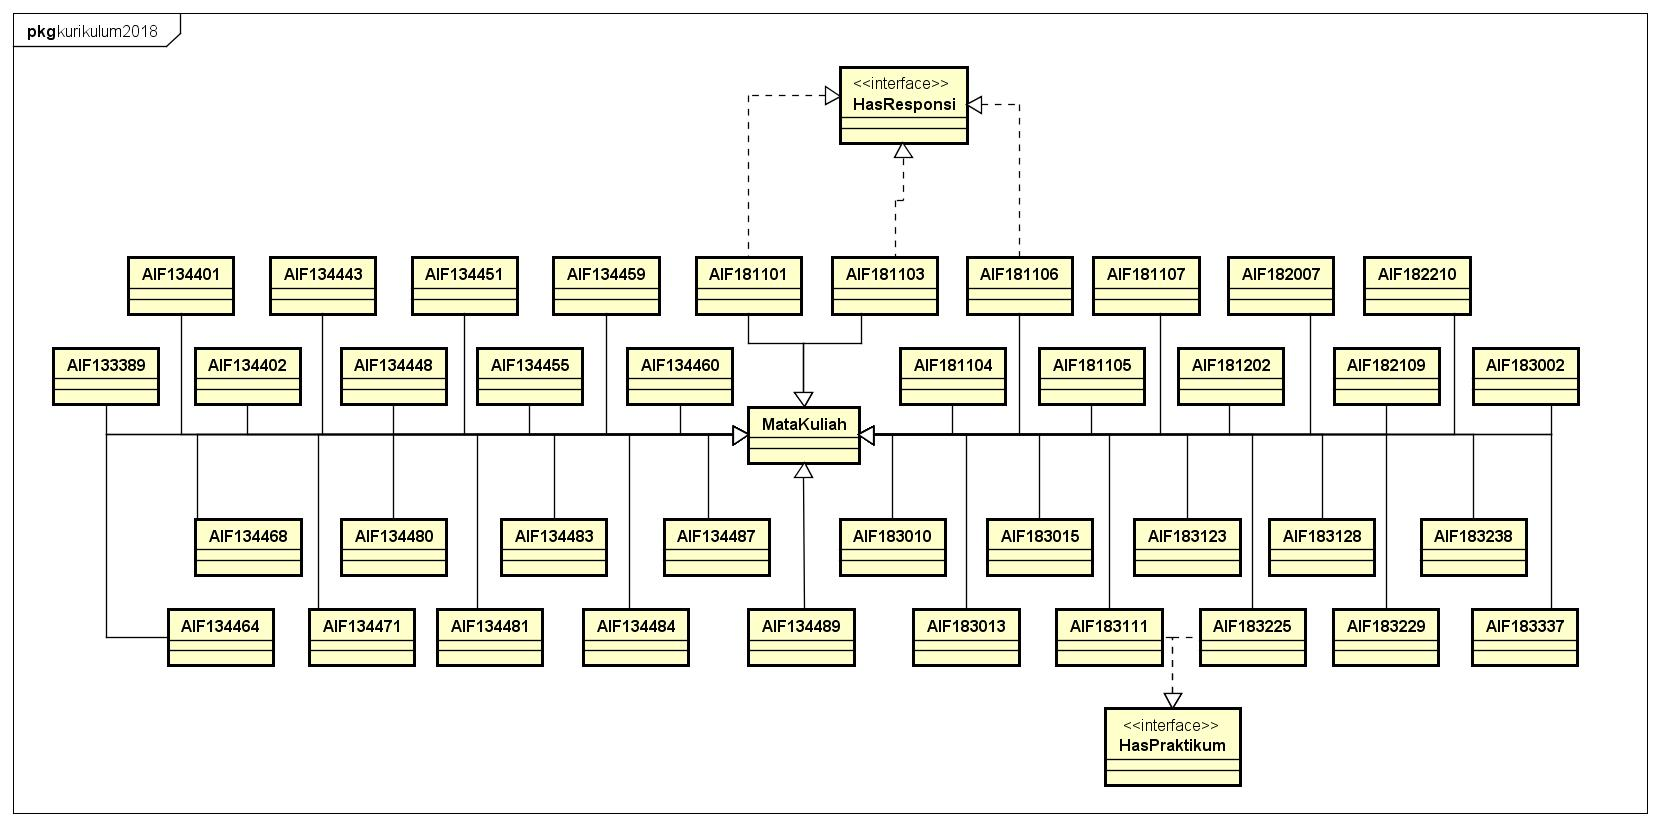
\includegraphics[scale=0.28]{Gambar/class-diagram-siamodels-mk-kurikulum-2018-2}
\caption{Diagram Kelas SIAModels \textit{Package} \texttt{kurikulum2018} (1/5)}
\label{fig:siamodels_class_2018_kurikulum_1}
\end{figure}

\begin{figure}[H]
\centering
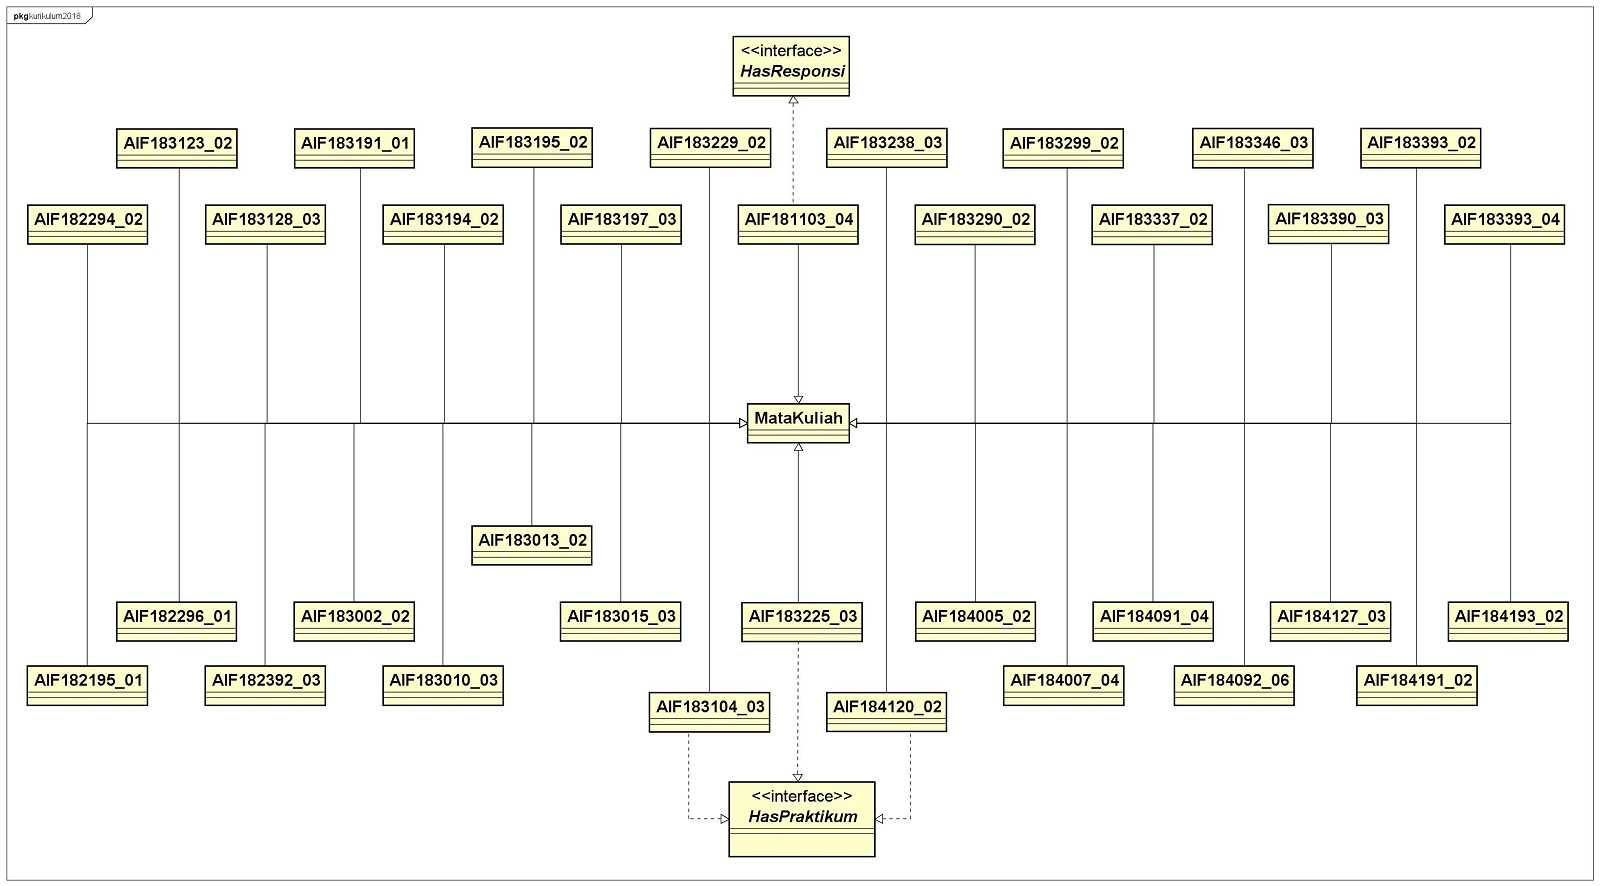
\includegraphics[scale=0.29]{Gambar/class-diagram-siamodels-mk-kurikulum-2018-1}
\caption{Diagram Kelas SIAModels \textit{Package} \texttt{kurikulum2018} (2/5)}
\label{fig:siamodels_class_2018_kurikulum_2}
\end{figure}

\begin{figure}[H]
\centering
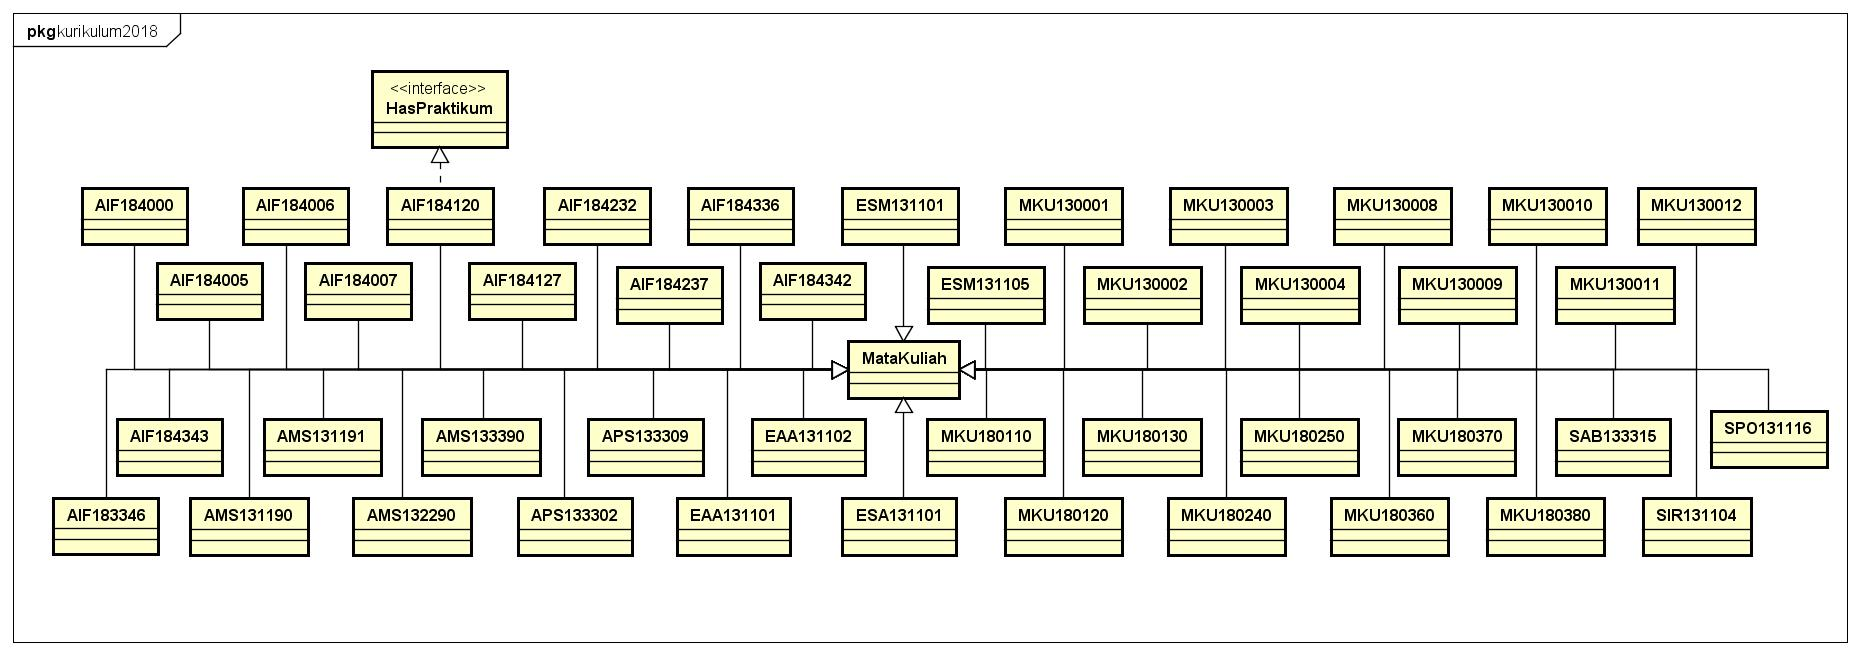
\includegraphics[scale=0.25]{Gambar/class-diagram-siamodels-mk-kurikulum-2018-3}
\caption{Diagram Kelas SIAModels \textit{Package} \texttt{kurikulum2018} (3/5)}
\label{fig:siamodels_class_2018_kurikulum_3}
\end{figure}

\begin{figure}[H]
\centering
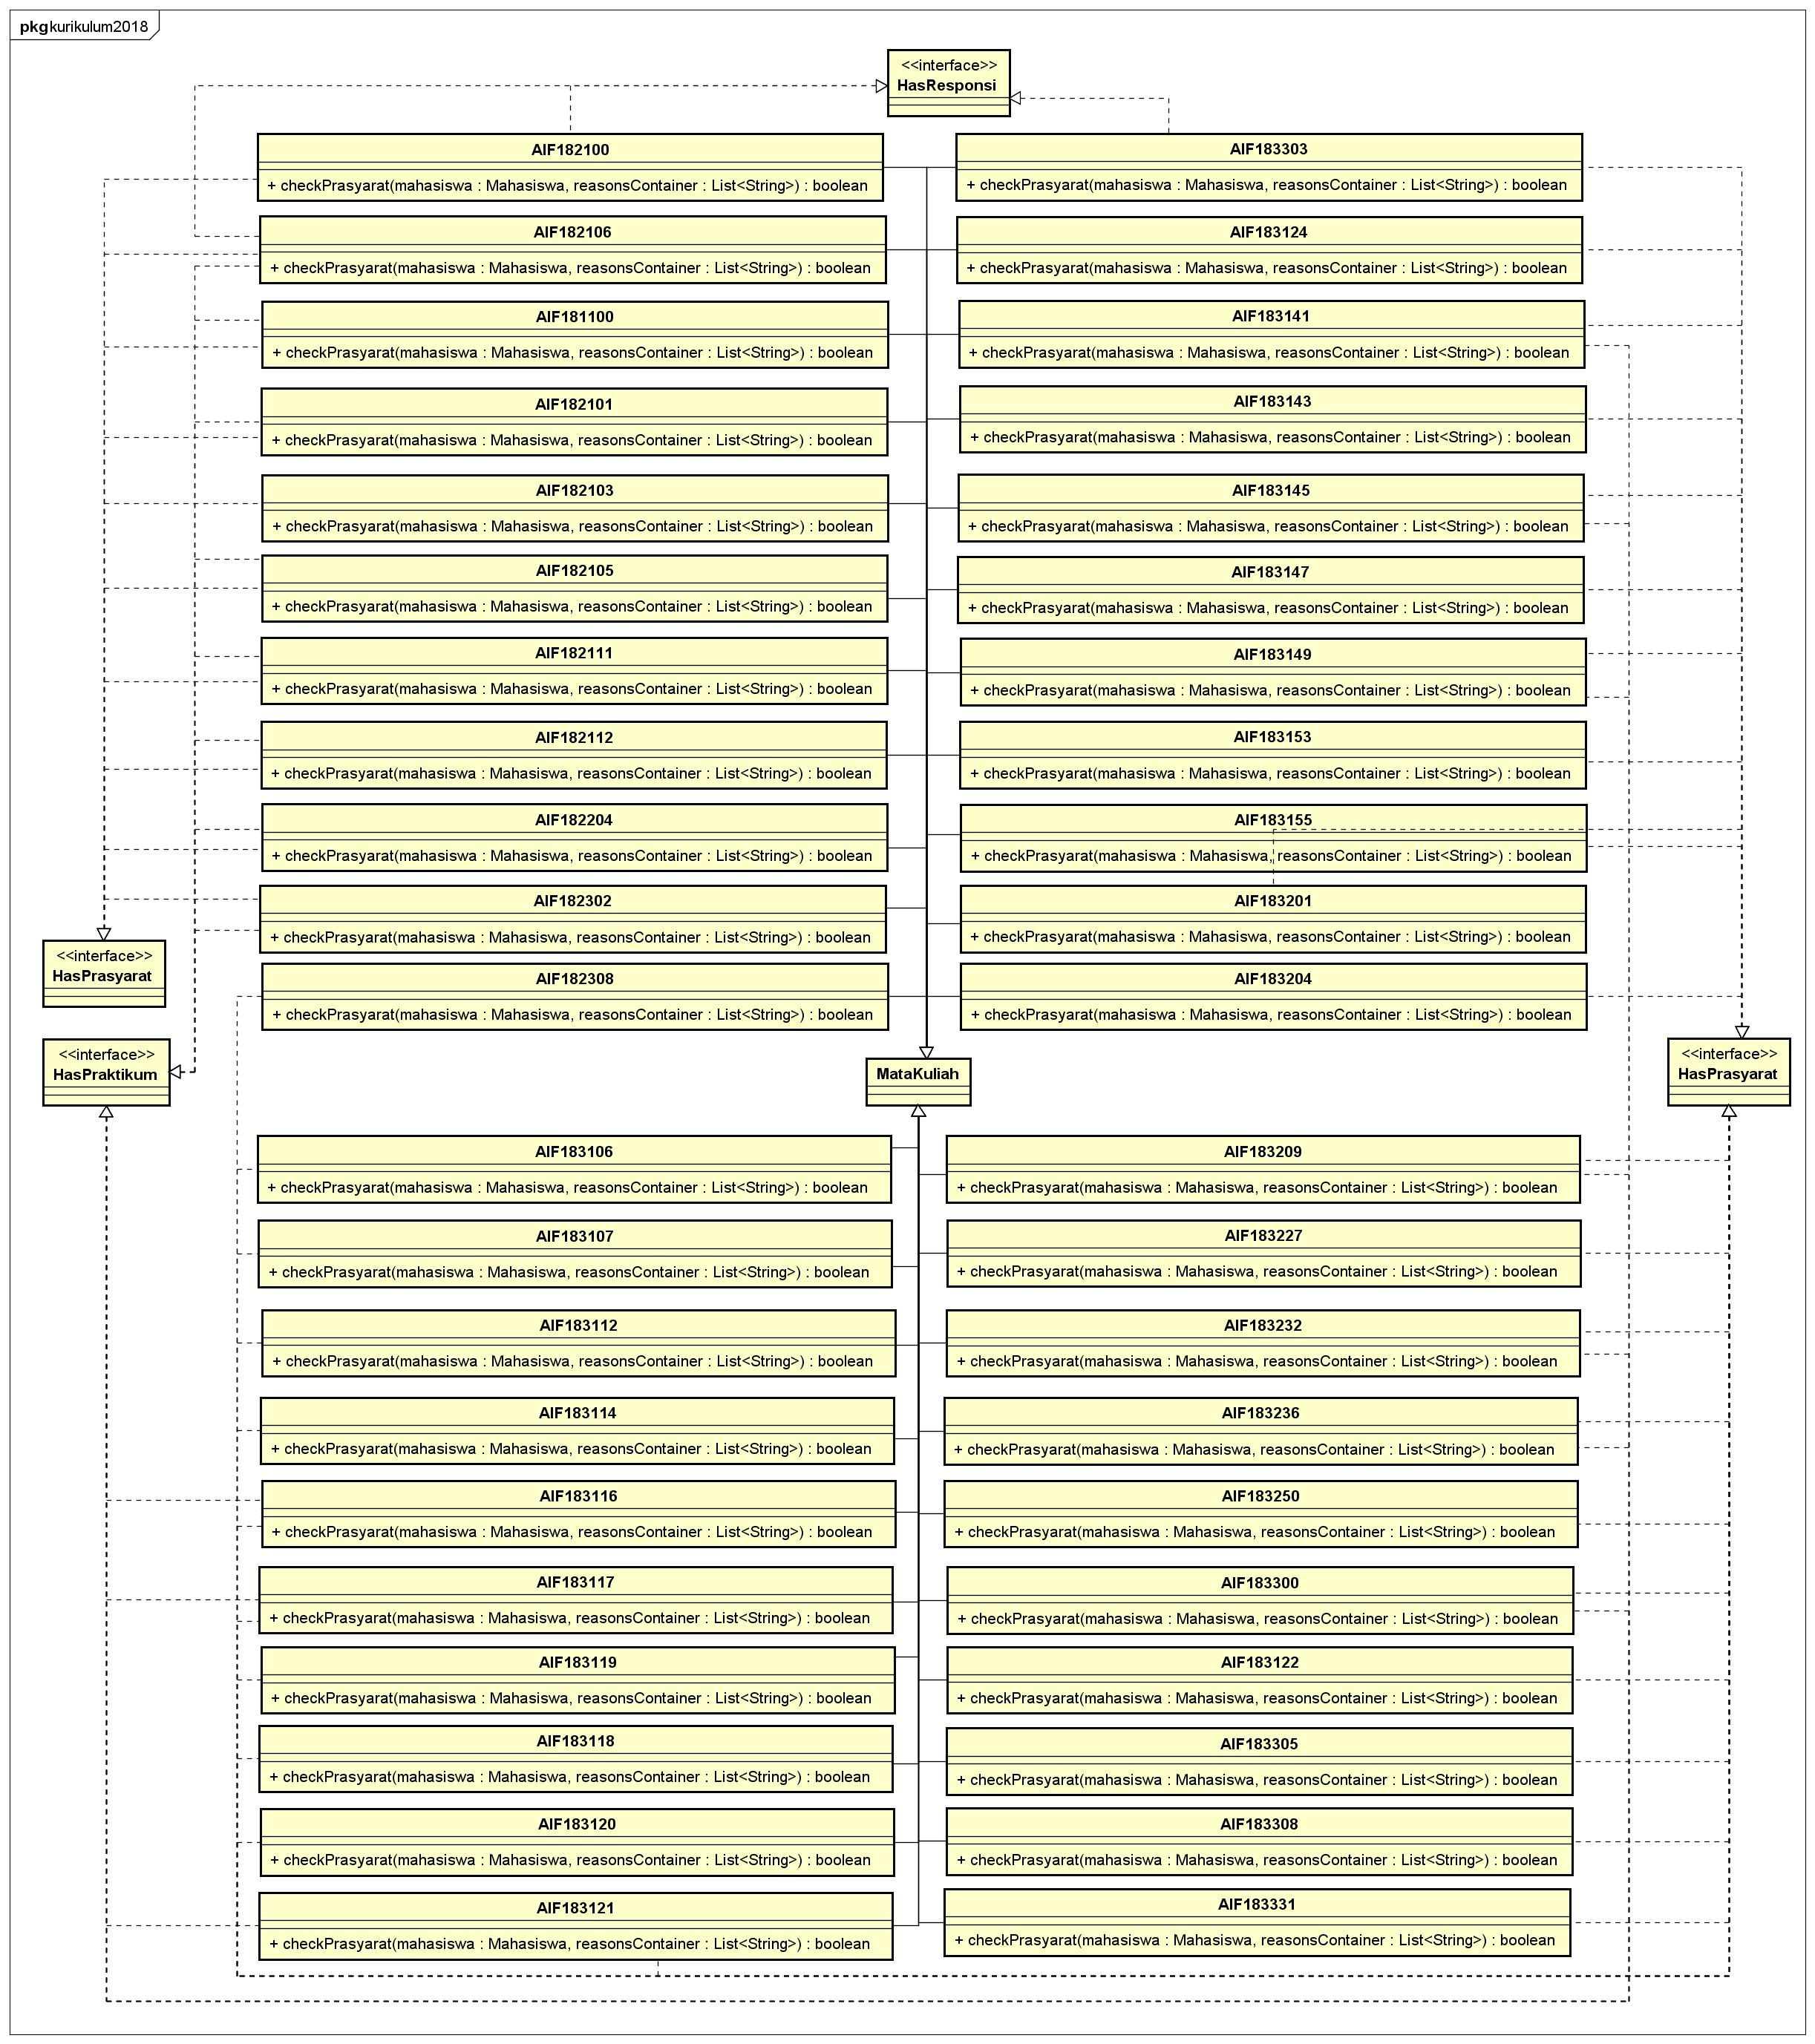
\includegraphics[scale=0.19]{Gambar/class-diagram-siamodels-mk-kurikulum-2018-4}
\caption{Diagram Kelas SIAModels \textit{Package} \texttt{kurikulum2018} (4/5)}
\label{fig:siamodels_class_2018_kurikulum_4}
\end{figure}

\begin{figure}[H]
\centering
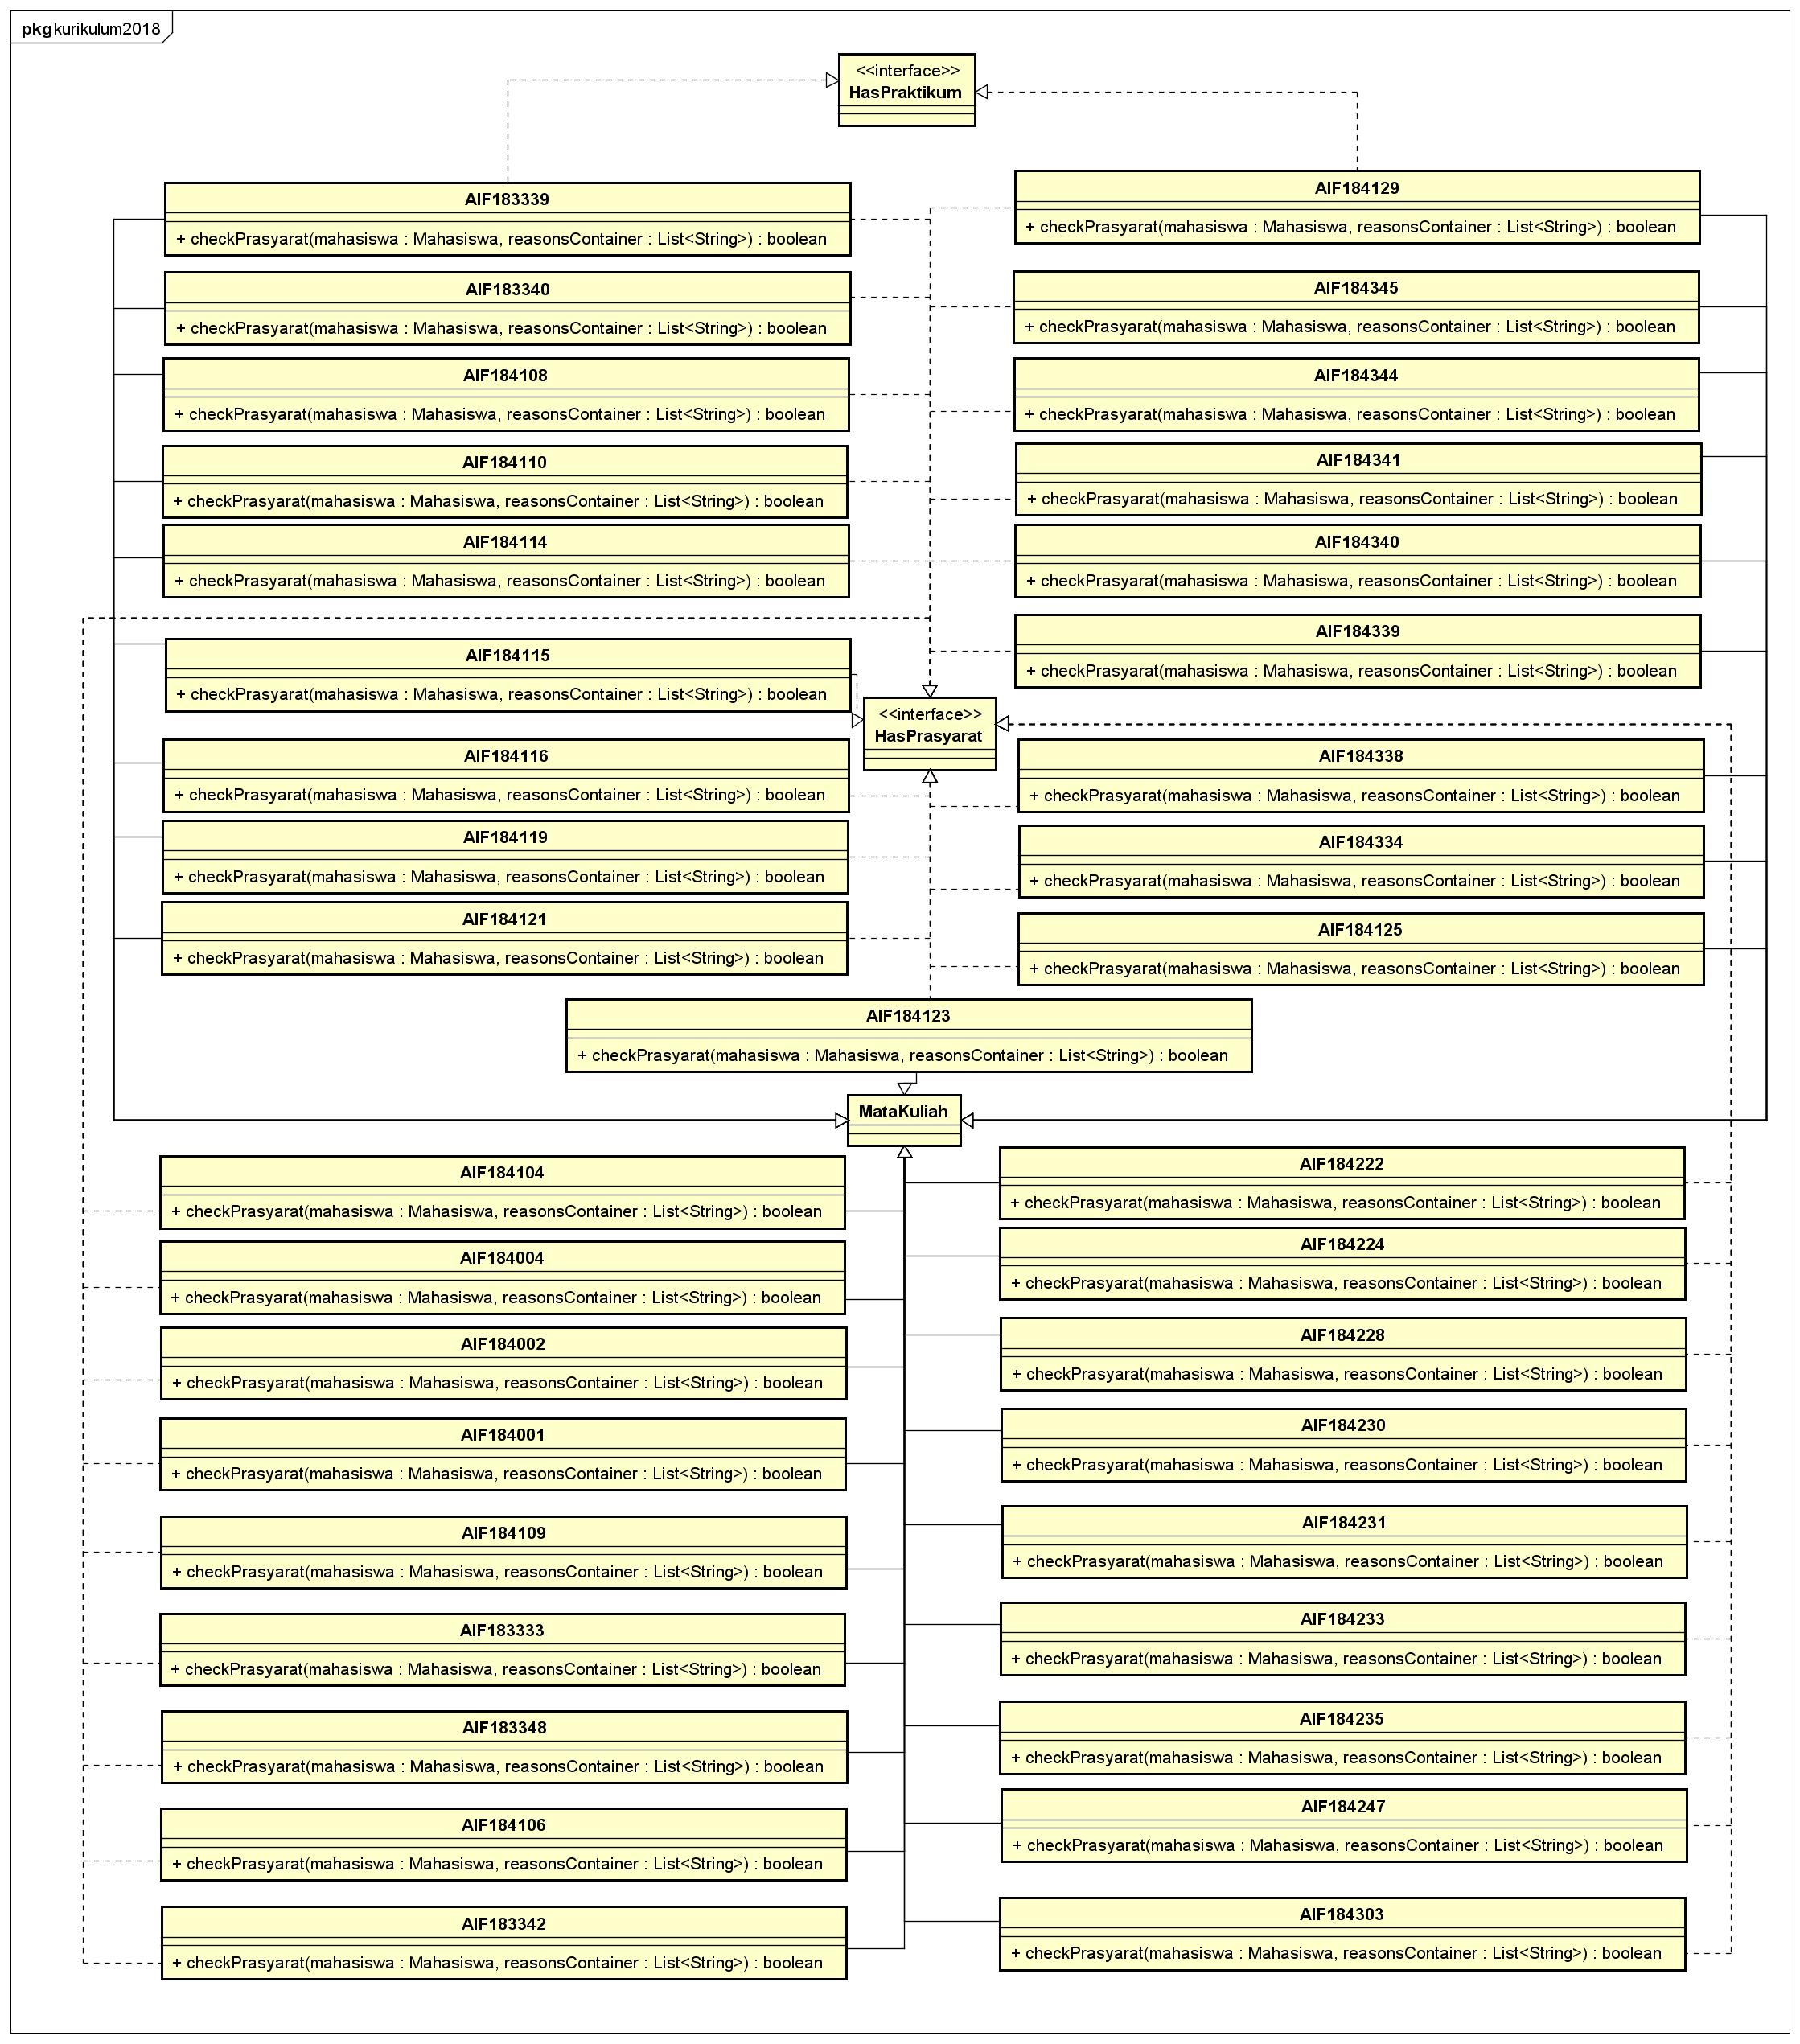
\includegraphics[scale=0.2]{Gambar/class-diagram-siamodels-mk-kurikulum-2018-5}
\caption{Diagram Kelas SIAModels \textit{Package} \texttt{kurikulum2018} (5/5)}
\label{fig:siamodels_class_2018_kurikulum_5}
\end{figure}

\begin{enumerate}
	\item \textit{Package} \texttt{id.ac.unpar.siamodels.matakuliah.kurikulum2018} \\
	\textit{Package} ini berisi kelas-kelas yang merepresentasikan mata kuliah pada kurikulum 2018 berserta aturan prasyaratnya. Kelas-kelas yang ada pada \textit{package} ini adalah sebagai berikut:
	\begin{itemize}
		\item \texttt{AIF131101} \\
Kelas ini merepresentasikan mata kuliah Pemrograman Berorientasi Objek.
\item \texttt{AIF131102} \\
Kelas ini merepresentasikan mata kuliah Algoritma dan Struktur Data.
\item \texttt{AIF131105} \\
Kelas ini merepresentasikan mata kuliah Pengantar Informatika.
\item \texttt{AIF131106} \\
Kelas ini merepresentasikan mata kuliah Sistem Dijital.
\item \texttt{AIF131181} \\
Kelas ini merepresentasikan mata kuliah Dasar-dasar Pemrograman.
\item \texttt{AIF131182} \\
Kelas ini merepresentasikan mata kuliah Pengantar Basis Data.
\item \texttt{AIF131183} \\
Kelas ini merepresentasikan mata kuliah Pemrograman Prosedural.
\item \texttt{AIF131191} \\
Kelas ini merepresentasikan mata kuliah Pemrograman Berorientasi Objek.
\item \texttt{AIF131192} \\
Kelas ini merepresentasikan mata kuliah Algoritma dan Struktur Data.
\item \texttt{AIF131195} \\
Kelas ini merepresentasikan mata kuliah Pengantar Informatika.
\item \texttt{AIF131198} \\
Kelas ini merepresentasikan mata kuliah Logika Informatika.
\item \texttt{AIF132202} \\
Kelas ini merepresentasikan mata kuliah Desain dan Analisis Algoritma.
\item \texttt{AIF132205} \\
Kelas ini merepresentasikan mata kuliah Arsitektur dan Organisasi Komputer.
\item \texttt{AIF132206} \\
Kelas ini merepresentasikan mata kuliah Sistem Operasi.
\item \texttt{AIF132208} \\
Kelas ini merepresentasikan mata kuliah Rekayasa Perangkat Lunak.
\item \texttt{AIF132210} \\
Kelas ini merepresentasikan mata kuliah Interaksi Manusia Komputer.
\item \texttt{AIF132280} \\
Kelas ini merepresentasikan mata kuliah Praktika Interaksi Manusia Komputer.
\item \texttt{AIF132281} \\
Kelas ini merepresentasikan mata kuliah Pengenalan Bidang Ilmu TIK.
\item \texttt{AIF132282} \\
Kelas ini merepresentasikan mata kuliah Algoritma dan Struktur Data Lanjut.
\item \texttt{AIF132290} \\
Kelas ini merepresentasikan mata kuliah Interaksi Manusia Komputer.
\item \texttt{AIF132291} \\
Kelas ini merepresentasikan mata kuliah Analisis dan Desain Berorientasi Objek.
\item \texttt{AIF132292} \\
Kelas ini merepresentasikan mata kuliah Desain dan Analisis Algoritma.
\item \texttt{AIF132294} \\
Kelas ini merepresentasikan mata kuliah Manajemen Informasi dan Basisdata.
\item \texttt{AIF132296} \\
Kelas ini merepresentasikan mata kuliah Sistem Operasi.
\item \texttt{AIF132298} \\
Kelas ini merepresentasikan mata kuliah Rekayasa Perangkat Lunak.
\item \texttt{AIF133305} \\
Kelas ini merepresentasikan mata kuliah Jaringan Komputer.
\item \texttt{AIF133315} \\
Kelas ini merepresentasikan mata kuliah Pemrograman Berbasis Web.
\item \texttt{AIF133317} \\
Kelas ini merepresentasikan mata kuliah Desain Antarmuka Grafis.
\item \texttt{AIF133318} \\
Kelas ini merepresentasikan mata kuliah Pemrograman Aplikasi Bergerak.
\item \texttt{AIF133337} \\
Kelas ini merepresentasikan mata kuliah Matematika Teknik.
\item \texttt{AIF133350} \\
Kelas ini merepresentasikan mata kuliah Algoritma Genetika.
\item \texttt{AIF133352} \\
Kelas ini merepresentasikan mata kuliah Jaringan Syaraf Tiruan.
\item \texttt{AIF133356} \\
Kelas ini merepresentasikan mata kuliah Analisis Proses Bisnis.
\item \texttt{AIF133380} \\
Kelas ini merepresentasikan mata kuliah Teori Bahasa dan Otomata.
\item \texttt{AIF133381} \\
Kelas ini merepresentasikan mata kuliah Analisis Sistem Informasi.
\item \texttt{AIF133382} \\
Kelas ini merepresentasikan mata kuliah Gudang Data dan Penambangan Data.
\item \texttt{AIF133383} \\
Kelas ini merepresentasikan mata kuliah Praktika Grafika Komputer.
\item \texttt{AIF133384} \\
Kelas ini merepresentasikan mata kuliah Praktika Pemrograman Basis Data.
\item \texttt{AIF133385} \\
Kelas ini merepresentasikan mata kuliah Praktika Pemrograman Berbasis Web.
\item \texttt{AIF133386} \\
Kelas ini merepresentasikan mata kuliah Manajemen Proyek Teknologi Informasi.
\item \texttt{AIF133388} \\
Kelas ini merepresentasikan mata kuliah Praktika Pemrograman Aplikasi Bergerak.
\item \texttt{AIF133389} \\
Kelas ini merepresentasikan mata kuliah Kriptografi.
\item \texttt{AIF134401} \\
Kelas ini merepresentasikan mata kuliah Skripsi 1.
\item \texttt{AIF134402} \\
Kelas ini merepresentasikan mata kuliah Skripsi 2.
\item \texttt{AIF134443} \\
Kelas ini merepresentasikan mata kuliah Matematika Kombinatorial.
\item \texttt{AIF134448} \\
Kelas ini merepresentasikan mata kuliah Pemrosesan Data Geografis.
\item \texttt{AIF134451} \\
Kelas ini merepresentasikan mata kuliah Audit Sistem Informasi.
\item \texttt{AIF134455} \\
Kelas ini merepresentasikan mata kuliah Sistem Pendukung Keputusan.
\item \texttt{AIF134459} \\
Kelas ini merepresentasikan mata kuliah Administrasi Basis Data.
\item \texttt{AIF134460} \\
Kelas ini merepresentasikan mata kuliah Manajemen Pengetahuan.
\item \texttt{AIF134464} \\
Kelas ini merepresentasikan mata kuliah Sistem Perusahaan Berskala Besar.
\item \texttt{AIF134468} \\
Kelas ini merepresentasikan mata kuliah Teknologi Multimedia.
\item \texttt{AIF134471} \\
Kelas ini merepresentasikan mata kuliah Metode Formal.
\item \texttt{AIF134480} \\
Kelas ini merepresentasikan mata kuliah Pemrograman Sistem.
\item \texttt{AIF134481} \\
Kelas ini merepresentasikan mata kuliah Sistem Pakar.
\item \texttt{AIF134483} \\
Kelas ini merepresentasikan mata kuliah Teknik Kompilasi.
\item \texttt{AIF134484} \\
Kelas ini merepresentasikan mata kuliah Kewirausahaan.
\item \texttt{AIF134487} \\
Kelas ini merepresentasikan mata kuliah Perencanaan Sistem Informasi.
\item \texttt{AIF134489} \\
Kelas ini merepresentasikan mata kuliah Keamanan Informasi Dijital.
\item \texttt{AIF181100} \\
Kelas ini merepresentasikan mata kuliah Dasar Pemrograman. Method yang dimiliki kelas ini adalah sebagai berikut: 
\begin{itemize}
\item \textbf{public boolean checkPrasyarat(Mahasiswa mahasiswa, List<String> reasonsContainer)}\\
Memeriksa prasyarat-prasyarat dari kuliah, spesifik untuk mahasiswa yang dituju. Jika ada pesan-pesan khusus, akan ditambahkan pada parameter reasonsContainer.\\
\textbf{Parameter:}
\begin{itemize}
\item \textbf{mahasiswa} prasyarat kuliah akan diperiksa spesifik pada mahasiswa ini.
\item \textbf{reasonsContainer} jika pesan-pesan terkait prasyarat akan ditambahkan di sini.
\end{itemize}
\textbf{Kembalian:} \texttt{true} jika seluruh prasyarat dipenuhi, \texttt{false} jika tidak.
\end{itemize}
\item \texttt{AIF181101} \\
Kelas ini merepresentasikan mata kuliah Pemodelan untuk Komputasi.
\item \texttt{AIF181103} \\
Kelas ini merepresentasikan mata kuliah Matematika Dasar.
\item \texttt{AIF181104} \\
Kelas ini merepresentasikan mata kuliah Logika Informatika.
\item \texttt{AIF181105} \\
Kelas ini merepresentasikan mata kuliah Pengantar Informatika.
\item \texttt{AIF181106} \\
Kelas ini merepresentasikan mata kuliah Matriks dan Ruang Vektor.
\item \texttt{AIF181107} \\
Kelas ini merepresentasikan mata kuliah Matematika Diskret.
\item \texttt{AIF181202} \\
Kelas ini merepresentasikan mata kuliah Arsitektur dan Organisasi Komputer.
\item \texttt{AIF182007} \\
Kelas ini merepresentasikan mata kuliah Teknik Presentasi.
\item \texttt{AIF182100} \\
Kelas ini merepresentasikan mata kuliah Analisis dan Desain Perangkat Lunak. Method yang dimiliki kelas ini adalah sebagai berikut: 
\begin{itemize}
\item \textbf{public boolean checkPrasyarat(Mahasiswa mahasiswa, List<String> reasonsContainer)}\\
Memeriksa prasyarat-prasyarat dari kuliah, spesifik untuk mahasiswa yang dituju. Jika ada pesan-pesan khusus, akan ditambahkan pada parameter reasonsContainer.\\
\textbf{Parameter:}
\begin{itemize}
\item \textbf{mahasiswa} prasyarat kuliah akan diperiksa spesifik pada mahasiswa ini.
\item \textbf{reasonsContainer} jika pesan-pesan terkait prasyarat akan ditambahkan di sini.
\end{itemize}
\textbf{Kembalian:} \texttt{true} jika seluruh prasyarat dipenuhi, \texttt{false} jika tidak.
\end{itemize}
\item \texttt{AIF182101} \\
Kelas ini merepresentasikan mata kuliah Algoritma dan Struktur Data. Method yang dimiliki kelas ini adalah sebagai berikut: 
\begin{itemize}
\item \textbf{public boolean checkPrasyarat(Mahasiswa mahasiswa, List<String> reasonsContainer)}\\
Memeriksa prasyarat-prasyarat dari kuliah, spesifik untuk mahasiswa yang dituju. Jika ada pesan-pesan khusus, akan ditambahkan pada parameter reasonsContainer.\\
\textbf{Parameter:}
\begin{itemize}
\item \textbf{mahasiswa} prasyarat kuliah akan diperiksa spesifik pada mahasiswa ini.
\item \textbf{reasonsContainer} jika pesan-pesan terkait prasyarat akan ditambahkan di sini.
\end{itemize}
\textbf{Kembalian:} \texttt{true} jika seluruh prasyarat dipenuhi, \texttt{false} jika tidak.
\end{itemize}
\item \texttt{AIF182103} \\
Kelas ini merepresentasikan mata kuliah Struktur Diskret. Method yang dimiliki kelas ini adalah sebagai berikut: 
\begin{itemize}
\item \textbf{public boolean checkPrasyarat(Mahasiswa mahasiswa, List<String> reasonsContainer)}\\
Memeriksa prasyarat-prasyarat dari kuliah, spesifik untuk mahasiswa yang dituju. Jika ada pesan-pesan khusus, akan ditambahkan pada parameter reasonsContainer.\\
\textbf{Parameter:}
\begin{itemize}
\item \textbf{mahasiswa} prasyarat kuliah akan diperiksa spesifik pada mahasiswa ini.
\item \textbf{reasonsContainer} jika pesan-pesan terkait prasyarat akan ditambahkan di sini.
\end{itemize}
\textbf{Kembalian:} \texttt{true} jika seluruh prasyarat dipenuhi, \texttt{false} jika tidak.
\end{itemize}
\item \texttt{AIF182105} \\
Kelas ini merepresentasikan mata kuliah Pemrograman Berorientasi Objek. Method yang dimiliki kelas ini adalah sebagai berikut: 
\begin{itemize}
\item \textbf{public boolean checkPrasyarat(Mahasiswa mahasiswa, List<String> reasonsContainer)}\\
Memeriksa prasyarat-prasyarat dari kuliah, spesifik untuk mahasiswa yang dituju. Jika ada pesan-pesan khusus, akan ditambahkan pada parameter reasonsContainer.\\
\textbf{Parameter:}
\begin{itemize}
\item \textbf{mahasiswa} prasyarat kuliah akan diperiksa spesifik pada mahasiswa ini.
\item \textbf{reasonsContainer} jika pesan-pesan terkait prasyarat akan ditambahkan di sini.
\end{itemize}
\textbf{Kembalian:} \texttt{true} jika seluruh prasyarat dipenuhi, \texttt{false} jika tidak.
\end{itemize}
\item \texttt{AIF182106} \\
Kelas ini merepresentasikan mata kuliah Desain dan Analisis Algoritma. Method yang dimiliki kelas ini adalah sebagai berikut: 
\begin{itemize}
\item \textbf{public boolean checkPrasyarat(Mahasiswa mahasiswa, List<String> reasonsContainer)}\\
Memeriksa prasyarat-prasyarat dari kuliah, spesifik untuk mahasiswa yang dituju. Jika ada pesan-pesan khusus, akan ditambahkan pada parameter reasonsContainer.\\
\textbf{Parameter:}
\begin{itemize}
\item \textbf{mahasiswa} prasyarat kuliah akan diperiksa spesifik pada mahasiswa ini.
\item \textbf{reasonsContainer} jika pesan-pesan terkait prasyarat akan ditambahkan di sini.
\end{itemize}
\textbf{Kembalian:} \texttt{true} jika seluruh prasyarat dipenuhi, \texttt{false} jika tidak.
\end{itemize}
\item \texttt{AIF182109} \\
Kelas ini merepresentasikan mata kuliah Statistika untuk Komputasi.
\item \texttt{AIF182111} \\
Kelas ini merepresentasikan mata kuliah Pemrograman Kompetitif 1. Method yang dimiliki kelas ini adalah sebagai berikut: 
\begin{itemize}
\item \textbf{public boolean checkPrasyarat(Mahasiswa mahasiswa, List<String> reasonsContainer)}\\
Memeriksa prasyarat-prasyarat dari kuliah, spesifik untuk mahasiswa yang dituju. Jika ada pesan-pesan khusus, akan ditambahkan pada parameter reasonsContainer.\\
\textbf{Parameter:}
\begin{itemize}
\item \textbf{mahasiswa} prasyarat kuliah akan diperiksa spesifik pada mahasiswa ini.
\item \textbf{reasonsContainer} jika pesan-pesan terkait prasyarat akan ditambahkan di sini.
\end{itemize}
\textbf{Kembalian:} \texttt{true} jika seluruh prasyarat dipenuhi, \texttt{false} jika tidak.
\end{itemize}
\item \texttt{AIF182112} \\
Kelas ini merepresentasikan mata kuliah Pemrograman Kompetitif 2. Method yang dimiliki kelas ini adalah sebagai berikut: 
\begin{itemize}
\item \textbf{public boolean checkPrasyarat(Mahasiswa mahasiswa, List<String> reasonsContainer)}\\
Memeriksa prasyarat-prasyarat dari kuliah, spesifik untuk mahasiswa yang dituju. Jika ada pesan-pesan khusus, akan ditambahkan pada parameter reasonsContainer.\\
\textbf{Parameter:}
\begin{itemize}
\item \textbf{mahasiswa} prasyarat kuliah akan diperiksa spesifik pada mahasiswa ini.
\item \textbf{reasonsContainer} jika pesan-pesan terkait prasyarat akan ditambahkan di sini.
\end{itemize}
\textbf{Kembalian:} \texttt{true} jika seluruh prasyarat dipenuhi, \texttt{false} jika tidak.
\end{itemize}
\item \texttt{AIF182204} \\
Kelas ini merepresentasikan mata kuliah Pemrograman Berbasis Web. Method yang dimiliki kelas ini adalah sebagai berikut: 
\begin{itemize}
\item \textbf{public boolean checkPrasyarat(Mahasiswa mahasiswa, List<String> reasonsContainer)}\\
Memeriksa prasyarat-prasyarat dari kuliah, spesifik untuk mahasiswa yang dituju. Jika ada pesan-pesan khusus, akan ditambahkan pada parameter reasonsContainer.\\
\textbf{Parameter:}
\begin{itemize}
\item \textbf{mahasiswa} prasyarat kuliah akan diperiksa spesifik pada mahasiswa ini.
\item \textbf{reasonsContainer} jika pesan-pesan terkait prasyarat akan ditambahkan di sini.
\end{itemize}
\textbf{Kembalian:} \texttt{true} jika seluruh prasyarat dipenuhi, \texttt{false} jika tidak.
\end{itemize}
\item \texttt{AIF182210} \\
Kelas ini merepresentasikan mata kuliah Pengantar Jaringan Komputer.
\item \texttt{AIF182302} \\
Kelas ini merepresentasikan mata kuliah Manajemen Informasi dan Basisdata. Method yang dimiliki kelas ini adalah sebagai berikut: 
\begin{itemize}
\item \textbf{public boolean checkPrasyarat(Mahasiswa mahasiswa, List<String> reasonsContainer)}\\
Memeriksa prasyarat-prasyarat dari kuliah, spesifik untuk mahasiswa yang dituju. Jika ada pesan-pesan khusus, akan ditambahkan pada parameter reasonsContainer.\\
\textbf{Parameter:}
\begin{itemize}
\item \textbf{mahasiswa} prasyarat kuliah akan diperiksa spesifik pada mahasiswa ini.
\item \textbf{reasonsContainer} jika pesan-pesan terkait prasyarat akan ditambahkan di sini.
\end{itemize}
\textbf{Kembalian:} \texttt{true} jika seluruh prasyarat dipenuhi, \texttt{false} jika tidak.
\end{itemize}
\item \texttt{AIF182308} \\
Kelas ini merepresentasikan mata kuliah Pengantar Sistem Informasi. Method yang dimiliki kelas ini adalah sebagai berikut: 
\begin{itemize}
\item \textbf{public boolean checkPrasyarat(Mahasiswa mahasiswa, List<String> reasonsContainer)}\\
Memeriksa prasyarat-prasyarat dari kuliah, spesifik untuk mahasiswa yang dituju. Jika ada pesan-pesan khusus, akan ditambahkan pada parameter reasonsContainer.\\
\textbf{Parameter:}
\begin{itemize}
\item \textbf{mahasiswa} prasyarat kuliah akan diperiksa spesifik pada mahasiswa ini.
\item \textbf{reasonsContainer} jika pesan-pesan terkait prasyarat akan ditambahkan di sini.
\end{itemize}
\textbf{Kembalian:} \texttt{true} jika seluruh prasyarat dipenuhi, \texttt{false} jika tidak.
\end{itemize}
\item \texttt{AIF183002} \\
Kelas ini merepresentasikan mata kuliah Penulisan Ilmiah.
\item \texttt{AIF183010} \\
Kelas ini merepresentasikan mata kuliah Kerja Praktek 2.
\item \texttt{AIF183013} \\
Kelas ini merepresentasikan mata kuliah Kerja Praktek 1.
\item \texttt{AIF183015} \\
Kelas ini merepresentasikan mata kuliah Pendidikan Pengabdian kepada Masyarakat.
\item \texttt{AIF183106} \\
Kelas ini merepresentasikan mata kuliah Proyek Informatika. Method yang dimiliki kelas ini adalah sebagai berikut: 
\begin{itemize}
\item \textbf{public boolean checkPrasyarat(Mahasiswa mahasiswa, List<String> reasonsContainer)}\\
Memeriksa prasyarat-prasyarat dari kuliah, spesifik untuk mahasiswa yang dituju. Jika ada pesan-pesan khusus, akan ditambahkan pada parameter reasonsContainer.\\
\textbf{Parameter:}
\begin{itemize}
\item \textbf{mahasiswa} prasyarat kuliah akan diperiksa spesifik pada mahasiswa ini.
\item \textbf{reasonsContainer} jika pesan-pesan terkait prasyarat akan ditambahkan di sini.
\end{itemize}
\textbf{Kembalian:} \texttt{true} jika seluruh prasyarat dipenuhi, \texttt{false} jika tidak.
\end{itemize}
\item \texttt{AIF183107} \\
Kelas ini merepresentasikan mata kuliah Pengantar Sistem Cerdas. Method yang dimiliki kelas ini adalah sebagai berikut: 
\begin{itemize}
\item \textbf{public boolean checkPrasyarat(Mahasiswa mahasiswa, List<String> reasonsContainer)}\\
Memeriksa prasyarat-prasyarat dari kuliah, spesifik untuk mahasiswa yang dituju. Jika ada pesan-pesan khusus, akan ditambahkan pada parameter reasonsContainer.\\
\textbf{Parameter:}
\begin{itemize}
\item \textbf{mahasiswa} prasyarat kuliah akan diperiksa spesifik pada mahasiswa ini.
\item \textbf{reasonsContainer} jika pesan-pesan terkait prasyarat akan ditambahkan di sini.
\end{itemize}
\textbf{Kembalian:} \texttt{true} jika seluruh prasyarat dipenuhi, \texttt{false} jika tidak.
\end{itemize}
\item \texttt{AIF183111} \\
Kelas ini merepresentasikan mata kuliah Interaksi Manusia Komputer.
\item \texttt{AIF183112} \\
Kelas ini merepresentasikan mata kuliah Pengujian Perangkat Lunak. Method yang dimiliki kelas ini adalah sebagai berikut: 
\begin{itemize}
\item \textbf{public boolean checkPrasyarat(Mahasiswa mahasiswa, List<String> reasonsContainer)}\\
Memeriksa prasyarat-prasyarat dari kuliah, spesifik untuk mahasiswa yang dituju. Jika ada pesan-pesan khusus, akan ditambahkan pada parameter reasonsContainer.\\
\textbf{Parameter:}
\begin{itemize}
\item \textbf{mahasiswa} prasyarat kuliah akan diperiksa spesifik pada mahasiswa ini.
\item \textbf{reasonsContainer} jika pesan-pesan terkait prasyarat akan ditambahkan di sini.
\end{itemize}
\textbf{Kembalian:} \texttt{true} jika seluruh prasyarat dipenuhi, \texttt{false} jika tidak.
\end{itemize}
\item \texttt{AIF183114} \\
Kelas ini merepresentasikan mata kuliah Algoritma Kriptografi. Method yang dimiliki kelas ini adalah sebagai berikut: 
\begin{itemize}
\item \textbf{public boolean checkPrasyarat(Mahasiswa mahasiswa, List<String> reasonsContainer)}\\
Memeriksa prasyarat-prasyarat dari kuliah, spesifik untuk mahasiswa yang dituju. Jika ada pesan-pesan khusus, akan ditambahkan pada parameter reasonsContainer.\\
\textbf{Parameter:}
\begin{itemize}
\item \textbf{mahasiswa} prasyarat kuliah akan diperiksa spesifik pada mahasiswa ini.
\item \textbf{reasonsContainer} jika pesan-pesan terkait prasyarat akan ditambahkan di sini.
\end{itemize}
\textbf{Kembalian:} \texttt{true} jika seluruh prasyarat dipenuhi, \texttt{false} jika tidak.
\end{itemize}
\item \texttt{AIF183116} \\
Kelas ini merepresentasikan mata kuliah Komputasi Paralel. Method yang dimiliki kelas ini adalah sebagai berikut: 
\begin{itemize}
\item \textbf{public boolean checkPrasyarat(Mahasiswa mahasiswa, List<String> reasonsContainer)}\\
Memeriksa prasyarat-prasyarat dari kuliah, spesifik untuk mahasiswa yang dituju. Jika ada pesan-pesan khusus, akan ditambahkan pada parameter reasonsContainer.\\
\textbf{Parameter:}
\begin{itemize}
\item \textbf{mahasiswa} prasyarat kuliah akan diperiksa spesifik pada mahasiswa ini.
\item \textbf{reasonsContainer} jika pesan-pesan terkait prasyarat akan ditambahkan di sini.
\end{itemize}
\textbf{Kembalian:} \texttt{true} jika seluruh prasyarat dipenuhi, \texttt{false} jika tidak.
\end{itemize}
\item \texttt{AIF183117} \\
Kelas ini merepresentasikan mata kuliah Grafika Komputer. Method yang dimiliki kelas ini adalah sebagai berikut: 
\begin{itemize}
\item \textbf{public boolean checkPrasyarat(Mahasiswa mahasiswa, List<String> reasonsContainer)}\\
Memeriksa prasyarat-prasyarat dari kuliah, spesifik untuk mahasiswa yang dituju. Jika ada pesan-pesan khusus, akan ditambahkan pada parameter reasonsContainer.\\
\textbf{Parameter:}
\begin{itemize}
\item \textbf{mahasiswa} prasyarat kuliah akan diperiksa spesifik pada mahasiswa ini.
\item \textbf{reasonsContainer} jika pesan-pesan terkait prasyarat akan ditambahkan di sini.
\end{itemize}
\textbf{Kembalian:} \texttt{true} jika seluruh prasyarat dipenuhi, \texttt{false} jika tidak.
\end{itemize}
\item \texttt{AIF183118} \\
Kelas ini merepresentasikan mata kuliah Komputasi Geometri. Method yang dimiliki kelas ini adalah sebagai berikut: 
\begin{itemize}
\item \textbf{public boolean checkPrasyarat(Mahasiswa mahasiswa, List<String> reasonsContainer)}\\
Memeriksa prasyarat-prasyarat dari kuliah, spesifik untuk mahasiswa yang dituju. Jika ada pesan-pesan khusus, akan ditambahkan pada parameter reasonsContainer.\\
\textbf{Parameter:}
\begin{itemize}
\item \textbf{mahasiswa} prasyarat kuliah akan diperiksa spesifik pada mahasiswa ini.
\item \textbf{reasonsContainer} jika pesan-pesan terkait prasyarat akan ditambahkan di sini.
\end{itemize}
\textbf{Kembalian:} \texttt{true} jika seluruh prasyarat dipenuhi, \texttt{false} jika tidak.
\end{itemize}
\item \texttt{AIF183119} \\
Kelas ini merepresentasikan mata kuliah Keamanan Informasi. Method yang dimiliki kelas ini adalah sebagai berikut: 
\begin{itemize}
\item \textbf{public boolean checkPrasyarat(Mahasiswa mahasiswa, List<String> reasonsContainer)}\\
Memeriksa prasyarat-prasyarat dari kuliah, spesifik untuk mahasiswa yang dituju. Jika ada pesan-pesan khusus, akan ditambahkan pada parameter reasonsContainer.\\
\textbf{Parameter:}
\begin{itemize}
\item \textbf{mahasiswa} prasyarat kuliah akan diperiksa spesifik pada mahasiswa ini.
\item \textbf{reasonsContainer} jika pesan-pesan terkait prasyarat akan ditambahkan di sini.
\end{itemize}
\textbf{Kembalian:} \texttt{true} jika seluruh prasyarat dipenuhi, \texttt{false} jika tidak.
\end{itemize}
\item \texttt{AIF183120} \\
Kelas ini merepresentasikan mata kuliah Perancangan Permainan Komputer. Method yang dimiliki kelas ini adalah sebagai berikut: 
\begin{itemize}
\item \textbf{public boolean checkPrasyarat(Mahasiswa mahasiswa, List<String> reasonsContainer)}\\
Memeriksa prasyarat-prasyarat dari kuliah, spesifik untuk mahasiswa yang dituju. Jika ada pesan-pesan khusus, akan ditambahkan pada parameter reasonsContainer.\\
\textbf{Parameter:}
\begin{itemize}
\item \textbf{mahasiswa} prasyarat kuliah akan diperiksa spesifik pada mahasiswa ini.
\item \textbf{reasonsContainer} jika pesan-pesan terkait prasyarat akan ditambahkan di sini.
\end{itemize}
\textbf{Kembalian:} \texttt{true} jika seluruh prasyarat dipenuhi, \texttt{false} jika tidak.
\end{itemize}
\item \texttt{AIF183121} \\
Kelas ini merepresentasikan mata kuliah Pemrograman Kompetitif 3. Method yang dimiliki kelas ini adalah sebagai berikut: 
\begin{itemize}
\item \textbf{public boolean checkPrasyarat(Mahasiswa mahasiswa, List<String> reasonsContainer)}\\
Memeriksa prasyarat-prasyarat dari kuliah, spesifik untuk mahasiswa yang dituju. Jika ada pesan-pesan khusus, akan ditambahkan pada parameter reasonsContainer.\\
\textbf{Parameter:}
\begin{itemize}
\item \textbf{mahasiswa} prasyarat kuliah akan diperiksa spesifik pada mahasiswa ini.
\item \textbf{reasonsContainer} jika pesan-pesan terkait prasyarat akan ditambahkan di sini.
\end{itemize}
\textbf{Kembalian:} \texttt{true} jika seluruh prasyarat dipenuhi, \texttt{false} jika tidak.
\end{itemize}
\item \texttt{AIF183122} \\
Kelas ini merepresentasikan mata kuliah Pemodelan \& Simulasi. Method yang dimiliki kelas ini adalah sebagai berikut: 
\begin{itemize}
\item \textbf{public boolean checkPrasyarat(Mahasiswa mahasiswa, List<String> reasonsContainer)}\\
Memeriksa prasyarat-prasyarat dari kuliah, spesifik untuk mahasiswa yang dituju. Jika ada pesan-pesan khusus, akan ditambahkan pada parameter reasonsContainer.\\
\textbf{Parameter:}
\begin{itemize}
\item \textbf{mahasiswa} prasyarat kuliah akan diperiksa spesifik pada mahasiswa ini.
\item \textbf{reasonsContainer} jika pesan-pesan terkait prasyarat akan ditambahkan di sini.
\end{itemize}
\textbf{Kembalian:} \texttt{true} jika seluruh prasyarat dipenuhi, \texttt{false} jika tidak.
\end{itemize}
\item \texttt{AIF183123} \\
Kelas ini merepresentasikan mata kuliah Topik Khusus Informatika 1.
\item \texttt{AIF183124} \\
Kelas ini merepresentasikan mata kuliah Grafika Komputer Lanjut. Method yang dimiliki kelas ini adalah sebagai berikut: 
\begin{itemize}
\item \textbf{public boolean checkPrasyarat(Mahasiswa mahasiswa, List<String> reasonsContainer)}\\
Memeriksa prasyarat-prasyarat dari kuliah, spesifik untuk mahasiswa yang dituju. Jika ada pesan-pesan khusus, akan ditambahkan pada parameter reasonsContainer.\\
\textbf{Parameter:}
\begin{itemize}
\item \textbf{mahasiswa} prasyarat kuliah akan diperiksa spesifik pada mahasiswa ini.
\item \textbf{reasonsContainer} jika pesan-pesan terkait prasyarat akan ditambahkan di sini.
\end{itemize}
\textbf{Kembalian:} \texttt{true} jika seluruh prasyarat dipenuhi, \texttt{false} jika tidak.
\end{itemize}
\item \texttt{AIF183128} \\
Kelas ini merepresentasikan mata kuliah Topik Khusus Informatika 2.
\item \texttt{AIF183141} \\
Kelas ini merepresentasikan mata kuliah Pemrograman Fungsional. Method yang dimiliki kelas ini adalah sebagai berikut: 
\begin{itemize}
\item \textbf{public boolean checkPrasyarat(Mahasiswa mahasiswa, List<String> reasonsContainer)}\\
Memeriksa prasyarat-prasyarat dari kuliah, spesifik untuk mahasiswa yang dituju. Jika ada pesan-pesan khusus, akan ditambahkan pada parameter reasonsContainer.\\
\textbf{Parameter:}
\begin{itemize}
\item \textbf{mahasiswa} prasyarat kuliah akan diperiksa spesifik pada mahasiswa ini.
\item \textbf{reasonsContainer} jika pesan-pesan terkait prasyarat akan ditambahkan di sini.
\end{itemize}
\textbf{Kembalian:} \texttt{true} jika seluruh prasyarat dipenuhi, \texttt{false} jika tidak.
\end{itemize}
\item \texttt{AIF183143} \\
Kelas ini merepresentasikan mata kuliah Pemodelan Formal. Method yang dimiliki kelas ini adalah sebagai berikut: 
\begin{itemize}
\item \textbf{public boolean checkPrasyarat(Mahasiswa mahasiswa, List<String> reasonsContainer)}\\
Memeriksa prasyarat-prasyarat dari kuliah, spesifik untuk mahasiswa yang dituju. Jika ada pesan-pesan khusus, akan ditambahkan pada parameter reasonsContainer.\\
\textbf{Parameter:}
\begin{itemize}
\item \textbf{mahasiswa} prasyarat kuliah akan diperiksa spesifik pada mahasiswa ini.
\item \textbf{reasonsContainer} jika pesan-pesan terkait prasyarat akan ditambahkan di sini.
\end{itemize}
\textbf{Kembalian:} \texttt{true} jika seluruh prasyarat dipenuhi, \texttt{false} jika tidak.
\end{itemize}
\item \texttt{AIF183145} \\
Kelas ini merepresentasikan mata kuliah Sertifikasi Dasar-dasar Java. Method yang dimiliki kelas ini adalah sebagai berikut: 
\begin{itemize}
\item \textbf{public boolean checkPrasyarat(Mahasiswa mahasiswa, List<String> reasonsContainer)}\\
Memeriksa prasyarat-prasyarat dari kuliah, spesifik untuk mahasiswa yang dituju. Jika ada pesan-pesan khusus, akan ditambahkan pada parameter reasonsContainer.\\
\textbf{Parameter:}
\begin{itemize}
\item \textbf{mahasiswa} prasyarat kuliah akan diperiksa spesifik pada mahasiswa ini.
\item \textbf{reasonsContainer} jika pesan-pesan terkait prasyarat akan ditambahkan di sini.
\end{itemize}
\textbf{Kembalian:} \texttt{true} jika seluruh prasyarat dipenuhi, \texttt{false} jika tidak.
\end{itemize}
\item \texttt{AIF183147} \\
Kelas ini merepresentasikan mata kuliah Teori Bilangan. Method yang dimiliki kelas ini adalah sebagai berikut: 
\begin{itemize}
\item \textbf{public boolean checkPrasyarat(Mahasiswa mahasiswa, List<String> reasonsContainer)}\\
Memeriksa prasyarat-prasyarat dari kuliah, spesifik untuk mahasiswa yang dituju. Jika ada pesan-pesan khusus, akan ditambahkan pada parameter reasonsContainer.\\
\textbf{Parameter:}
\begin{itemize}
\item \textbf{mahasiswa} prasyarat kuliah akan diperiksa spesifik pada mahasiswa ini.
\item \textbf{reasonsContainer} jika pesan-pesan terkait prasyarat akan ditambahkan di sini.
\end{itemize}
\textbf{Kembalian:} \texttt{true} jika seluruh prasyarat dipenuhi, \texttt{false} jika tidak.
\end{itemize}
\item \texttt{AIF183149} \\
Kelas ini merepresentasikan mata kuliah Teori Bahasa \& Kompilasi. Method yang dimiliki kelas ini adalah sebagai berikut: 
\begin{itemize}
\item \textbf{public boolean checkPrasyarat(Mahasiswa mahasiswa, List<String> reasonsContainer)}\\
Memeriksa prasyarat-prasyarat dari kuliah, spesifik untuk mahasiswa yang dituju. Jika ada pesan-pesan khusus, akan ditambahkan pada parameter reasonsContainer.\\
\textbf{Parameter:}
\begin{itemize}
\item \textbf{mahasiswa} prasyarat kuliah akan diperiksa spesifik pada mahasiswa ini.
\item \textbf{reasonsContainer} jika pesan-pesan terkait prasyarat akan ditambahkan di sini.
\end{itemize}
\textbf{Kembalian:} \texttt{true} jika seluruh prasyarat dipenuhi, \texttt{false} jika tidak.
\end{itemize}
\item \texttt{AIF183153} \\
Kelas ini merepresentasikan mata kuliah Metode Numerik. Method yang dimiliki kelas ini adalah sebagai berikut: 
\begin{itemize}
\item \textbf{public boolean checkPrasyarat(Mahasiswa mahasiswa, List<String> reasonsContainer)}\\
Memeriksa prasyarat-prasyarat dari kuliah, spesifik untuk mahasiswa yang dituju. Jika ada pesan-pesan khusus, akan ditambahkan pada parameter reasonsContainer.\\
\textbf{Parameter:}
\begin{itemize}
\item \textbf{mahasiswa} prasyarat kuliah akan diperiksa spesifik pada mahasiswa ini.
\item \textbf{reasonsContainer} jika pesan-pesan terkait prasyarat akan ditambahkan di sini.
\end{itemize}
\textbf{Kembalian:} \texttt{true} jika seluruh prasyarat dipenuhi, \texttt{false} jika tidak.
\end{itemize}
\item \texttt{AIF183155} \\
Kelas ini merepresentasikan mata kuliah Pemrograman Lojik. Method yang dimiliki kelas ini adalah sebagai berikut: 
\begin{itemize}
\item \textbf{public boolean checkPrasyarat(Mahasiswa mahasiswa, List<String> reasonsContainer)}\\
Memeriksa prasyarat-prasyarat dari kuliah, spesifik untuk mahasiswa yang dituju. Jika ada pesan-pesan khusus, akan ditambahkan pada parameter reasonsContainer.\\
\textbf{Parameter:}
\begin{itemize}
\item \textbf{mahasiswa} prasyarat kuliah akan diperiksa spesifik pada mahasiswa ini.
\item \textbf{reasonsContainer} jika pesan-pesan terkait prasyarat akan ditambahkan di sini.
\end{itemize}
\textbf{Kembalian:} \texttt{true} jika seluruh prasyarat dipenuhi, \texttt{false} jika tidak.
\end{itemize}
\item \texttt{AIF183201} \\
Kelas ini merepresentasikan mata kuliah Sistem Operasi. Method yang dimiliki kelas ini adalah sebagai berikut: 
\begin{itemize}
\item \textbf{public boolean checkPrasyarat(Mahasiswa mahasiswa, List<String> reasonsContainer)}\\
Memeriksa prasyarat-prasyarat dari kuliah, spesifik untuk mahasiswa yang dituju. Jika ada pesan-pesan khusus, akan ditambahkan pada parameter reasonsContainer.\\
\textbf{Parameter:}
\begin{itemize}
\item \textbf{mahasiswa} prasyarat kuliah akan diperiksa spesifik pada mahasiswa ini.
\item \textbf{reasonsContainer} jika pesan-pesan terkait prasyarat akan ditambahkan di sini.
\end{itemize}
\textbf{Kembalian:} \texttt{true} jika seluruh prasyarat dipenuhi, \texttt{false} jika tidak.
\end{itemize}
\item \texttt{AIF183204} \\
Kelas ini merepresentasikan mata kuliah Jaringan Komputer. Method yang dimiliki kelas ini adalah sebagai berikut: 
\begin{itemize}
\item \textbf{public boolean checkPrasyarat(Mahasiswa mahasiswa, List<String> reasonsContainer)}\\
Memeriksa prasyarat-prasyarat dari kuliah, spesifik untuk mahasiswa yang dituju. Jika ada pesan-pesan khusus, akan ditambahkan pada parameter reasonsContainer.\\
\textbf{Parameter:}
\begin{itemize}
\item \textbf{mahasiswa} prasyarat kuliah akan diperiksa spesifik pada mahasiswa ini.
\item \textbf{reasonsContainer} jika pesan-pesan terkait prasyarat akan ditambahkan di sini.
\end{itemize}
\textbf{Kembalian:} \texttt{true} jika seluruh prasyarat dipenuhi, \texttt{false} jika tidak.
\end{itemize}
\item \texttt{AIF183209} \\
Kelas ini merepresentasikan mata kuliah Pemrograman pada Perangkat Bergerak. Method yang dimiliki kelas ini adalah sebagai berikut: 
\begin{itemize}
\item \textbf{public boolean checkPrasyarat(Mahasiswa mahasiswa, List<String> reasonsContainer)}\\
Memeriksa prasyarat-prasyarat dari kuliah, spesifik untuk mahasiswa yang dituju. Jika ada pesan-pesan khusus, akan ditambahkan pada parameter reasonsContainer.\\
\textbf{Parameter:}
\begin{itemize}
\item \textbf{mahasiswa} prasyarat kuliah akan diperiksa spesifik pada mahasiswa ini.
\item \textbf{reasonsContainer} jika pesan-pesan terkait prasyarat akan ditambahkan di sini.
\end{itemize}
\textbf{Kembalian:} \texttt{true} jika seluruh prasyarat dipenuhi, \texttt{false} jika tidak.
\end{itemize}
\item \texttt{AIF183225} \\
Kelas ini merepresentasikan mata kuliah Seritifikasi Administrasi Jaringan Komputer 1.
\item \texttt{AIF183227} \\
Kelas ini merepresentasikan mata kuliah Pengantar Telekomunikasi. Method yang dimiliki kelas ini adalah sebagai berikut: 
\begin{itemize}
\item \textbf{public boolean checkPrasyarat(Mahasiswa mahasiswa, List<String> reasonsContainer)}\\
Memeriksa prasyarat-prasyarat dari kuliah, spesifik untuk mahasiswa yang dituju. Jika ada pesan-pesan khusus, akan ditambahkan pada parameter reasonsContainer.\\
\textbf{Parameter:}
\begin{itemize}
\item \textbf{mahasiswa} prasyarat kuliah akan diperiksa spesifik pada mahasiswa ini.
\item \textbf{reasonsContainer} jika pesan-pesan terkait prasyarat akan ditambahkan di sini.
\end{itemize}
\textbf{Kembalian:} \texttt{true} jika seluruh prasyarat dipenuhi, \texttt{false} jika tidak.
\end{itemize}
\item \texttt{AIF183229} \\
Kelas ini merepresentasikan mata kuliah Topik Khusus Sistem Terdistribusi 1.
\item \texttt{AIF183232} \\
Kelas ini merepresentasikan mata kuliah Pemrograman Berbasis Web Lanjut. Method yang dimiliki kelas ini adalah sebagai berikut: 
\begin{itemize}
\item \textbf{public boolean checkPrasyarat(Mahasiswa mahasiswa, List<String> reasonsContainer)}\\
Memeriksa prasyarat-prasyarat dari kuliah, spesifik untuk mahasiswa yang dituju. Jika ada pesan-pesan khusus, akan ditambahkan pada parameter reasonsContainer.\\
\textbf{Parameter:}
\begin{itemize}
\item \textbf{mahasiswa} prasyarat kuliah akan diperiksa spesifik pada mahasiswa ini.
\item \textbf{reasonsContainer} jika pesan-pesan terkait prasyarat akan ditambahkan di sini.
\end{itemize}
\textbf{Kembalian:} \texttt{true} jika seluruh prasyarat dipenuhi, \texttt{false} jika tidak.
\end{itemize}
\item \texttt{AIF183236} \\
Kelas ini merepresentasikan mata kuliah Seritifikasi Administrasi Jaringan Komputer 2. Method yang dimiliki kelas ini adalah sebagai berikut: 
\begin{itemize}
\item \textbf{public boolean checkPrasyarat(Mahasiswa mahasiswa, List<String> reasonsContainer)}\\
Memeriksa prasyarat-prasyarat dari kuliah, spesifik untuk mahasiswa yang dituju. Jika ada pesan-pesan khusus, akan ditambahkan pada parameter reasonsContainer.\\
\textbf{Parameter:}
\begin{itemize}
\item \textbf{mahasiswa} prasyarat kuliah akan diperiksa spesifik pada mahasiswa ini.
\item \textbf{reasonsContainer} jika pesan-pesan terkait prasyarat akan ditambahkan di sini.
\end{itemize}
\textbf{Kembalian:} \texttt{true} jika seluruh prasyarat dipenuhi, \texttt{false} jika tidak.
\end{itemize}
\item \texttt{AIF183238} \\
Kelas ini merepresentasikan mata kuliah Topik Khusus Sistem Terdistribusi 2.
\item \texttt{AIF183250} \\
Kelas ini merepresentasikan mata kuliah Sistem \& Aplikasi Telematika. Method yang dimiliki kelas ini adalah sebagai berikut: 
\begin{itemize}
\item \textbf{public boolean checkPrasyarat(Mahasiswa mahasiswa, List<String> reasonsContainer)}\\
Memeriksa prasyarat-prasyarat dari kuliah, spesifik untuk mahasiswa yang dituju. Jika ada pesan-pesan khusus, akan ditambahkan pada parameter reasonsContainer.\\
\textbf{Parameter:}
\begin{itemize}
\item \textbf{mahasiswa} prasyarat kuliah akan diperiksa spesifik pada mahasiswa ini.
\item \textbf{reasonsContainer} jika pesan-pesan terkait prasyarat akan ditambahkan di sini.
\end{itemize}
\textbf{Kembalian:} \texttt{true} jika seluruh prasyarat dipenuhi, \texttt{false} jika tidak.
\end{itemize}
\item \texttt{AIF183300} \\
Kelas ini merepresentasikan mata kuliah Teknologi Basisdata. Method yang dimiliki kelas ini adalah sebagai berikut: 
\begin{itemize}
\item \textbf{public boolean checkPrasyarat(Mahasiswa mahasiswa, List<String> reasonsContainer)}\\
Memeriksa prasyarat-prasyarat dari kuliah, spesifik untuk mahasiswa yang dituju. Jika ada pesan-pesan khusus, akan ditambahkan pada parameter reasonsContainer.\\
\textbf{Parameter:}
\begin{itemize}
\item \textbf{mahasiswa} prasyarat kuliah akan diperiksa spesifik pada mahasiswa ini.
\item \textbf{reasonsContainer} jika pesan-pesan terkait prasyarat akan ditambahkan di sini.
\end{itemize}
\textbf{Kembalian:} \texttt{true} jika seluruh prasyarat dipenuhi, \texttt{false} jika tidak.
\end{itemize}
\item \texttt{AIF183303} \\
Kelas ini merepresentasikan mata kuliah Rekayasa Perangkat Lunak. Method yang dimiliki kelas ini adalah sebagai berikut: 
\begin{itemize}
\item \textbf{public boolean checkPrasyarat(Mahasiswa mahasiswa, List<String> reasonsContainer)}\\
Memeriksa prasyarat-prasyarat dari kuliah, spesifik untuk mahasiswa yang dituju. Jika ada pesan-pesan khusus, akan ditambahkan pada parameter reasonsContainer.\\
\textbf{Parameter:}
\begin{itemize}
\item \textbf{mahasiswa} prasyarat kuliah akan diperiksa spesifik pada mahasiswa ini.
\item \textbf{reasonsContainer} jika pesan-pesan terkait prasyarat akan ditambahkan di sini.
\end{itemize}
\textbf{Kembalian:} \texttt{true} jika seluruh prasyarat dipenuhi, \texttt{false} jika tidak.
\end{itemize}
\item \texttt{AIF183305} \\
Kelas ini merepresentasikan mata kuliah Manajemen Proyek. Method yang dimiliki kelas ini adalah sebagai berikut: 
\begin{itemize}
\item \textbf{public boolean checkPrasyarat(Mahasiswa mahasiswa, List<String> reasonsContainer)}\\
Memeriksa prasyarat-prasyarat dari kuliah, spesifik untuk mahasiswa yang dituju. Jika ada pesan-pesan khusus, akan ditambahkan pada parameter reasonsContainer.\\
\textbf{Parameter:}
\begin{itemize}
\item \textbf{mahasiswa} prasyarat kuliah akan diperiksa spesifik pada mahasiswa ini.
\item \textbf{reasonsContainer} jika pesan-pesan terkait prasyarat akan ditambahkan di sini.
\end{itemize}
\textbf{Kembalian:} \texttt{true} jika seluruh prasyarat dipenuhi, \texttt{false} jika tidak.
\end{itemize}
\item \texttt{AIF183308} \\
Kelas ini merepresentasikan mata kuliah Proyek Sistem Informasi 1. Method yang dimiliki kelas ini adalah sebagai berikut: 
\begin{itemize}
\item \textbf{public boolean checkPrasyarat(Mahasiswa mahasiswa, List<String> reasonsContainer)}\\
Memeriksa prasyarat-prasyarat dari kuliah, spesifik untuk mahasiswa yang dituju. Jika ada pesan-pesan khusus, akan ditambahkan pada parameter reasonsContainer.\\
\textbf{Parameter:}
\begin{itemize}
\item \textbf{mahasiswa} prasyarat kuliah akan diperiksa spesifik pada mahasiswa ini.
\item \textbf{reasonsContainer} jika pesan-pesan terkait prasyarat akan ditambahkan di sini.
\end{itemize}
\textbf{Kembalian:} \texttt{true} jika seluruh prasyarat dipenuhi, \texttt{false} jika tidak.
\end{itemize}
\item \texttt{AIF183331} \\
Kelas ini merepresentasikan mata kuliah Sistem e-Commerce. Method yang dimiliki kelas ini adalah sebagai berikut: 
\begin{itemize}
\item \textbf{public boolean checkPrasyarat(Mahasiswa mahasiswa, List<String> reasonsContainer)}\\
Memeriksa prasyarat-prasyarat dari kuliah, spesifik untuk mahasiswa yang dituju. Jika ada pesan-pesan khusus, akan ditambahkan pada parameter reasonsContainer.\\
\textbf{Parameter:}
\begin{itemize}
\item \textbf{mahasiswa} prasyarat kuliah akan diperiksa spesifik pada mahasiswa ini.
\item \textbf{reasonsContainer} jika pesan-pesan terkait prasyarat akan ditambahkan di sini.
\end{itemize}
\textbf{Kembalian:} \texttt{true} jika seluruh prasyarat dipenuhi, \texttt{false} jika tidak.
\end{itemize}
\item \texttt{AIF183333} \\
Kelas ini merepresentasikan mata kuliah Metodologi Pengembangan Sistem Informasi 1. Method yang dimiliki kelas ini adalah sebagai berikut: 
\begin{itemize}
\item \textbf{public boolean checkPrasyarat(Mahasiswa mahasiswa, List<String> reasonsContainer)}\\
Memeriksa prasyarat-prasyarat dari kuliah, spesifik untuk mahasiswa yang dituju. Jika ada pesan-pesan khusus, akan ditambahkan pada parameter reasonsContainer.\\
\textbf{Parameter:}
\begin{itemize}
\item \textbf{mahasiswa} prasyarat kuliah akan diperiksa spesifik pada mahasiswa ini.
\item \textbf{reasonsContainer} jika pesan-pesan terkait prasyarat akan ditambahkan di sini.
\end{itemize}
\textbf{Kembalian:} \texttt{true} jika seluruh prasyarat dipenuhi, \texttt{false} jika tidak.
\end{itemize}
\item \texttt{AIF183337} \\
Kelas ini merepresentasikan mata kuliah Topik Khusus Sistem Informasi 1.
\item \texttt{AIF183339} \\
Kelas ini merepresentasikan mata kuliah Sertifikasi Perancangan dan Pemrograman Basis Data dengan SQL. Method yang dimiliki kelas ini adalah sebagai berikut: 
\begin{itemize}
\item \textbf{public boolean checkPrasyarat(Mahasiswa mahasiswa, List<String> reasonsContainer)}\\
Memeriksa prasyarat-prasyarat dari kuliah, spesifik untuk mahasiswa yang dituju. Jika ada pesan-pesan khusus, akan ditambahkan pada parameter reasonsContainer.\\
\textbf{Parameter:}
\begin{itemize}
\item \textbf{mahasiswa} prasyarat kuliah akan diperiksa spesifik pada mahasiswa ini.
\item \textbf{reasonsContainer} jika pesan-pesan terkait prasyarat akan ditambahkan di sini.
\end{itemize}
\textbf{Kembalian:} \texttt{true} jika seluruh prasyarat dipenuhi, \texttt{false} jika tidak.
\end{itemize}
\item \texttt{AIF183340} \\
Kelas ini merepresentasikan mata kuliah Metodologi Pengembangan Sistem Informasi 2. Method yang dimiliki kelas ini adalah sebagai berikut: 
\begin{itemize}
\item \textbf{public boolean checkPrasyarat(Mahasiswa mahasiswa, List<String> reasonsContainer)}\\
Memeriksa prasyarat-prasyarat dari kuliah, spesifik untuk mahasiswa yang dituju. Jika ada pesan-pesan khusus, akan ditambahkan pada parameter reasonsContainer.\\
\textbf{Parameter:}
\begin{itemize}
\item \textbf{mahasiswa} prasyarat kuliah akan diperiksa spesifik pada mahasiswa ini.
\item \textbf{reasonsContainer} jika pesan-pesan terkait prasyarat akan ditambahkan di sini.
\end{itemize}
\textbf{Kembalian:} \texttt{true} jika seluruh prasyarat dipenuhi, \texttt{false} jika tidak.
\end{itemize}
\item \texttt{AIF183342} \\
Kelas ini merepresentasikan mata kuliah Kewirausahaan Berbasis Teknologi. Method yang dimiliki kelas ini adalah sebagai berikut: 
\begin{itemize}
\item \textbf{public boolean checkPrasyarat(Mahasiswa mahasiswa, List<String> reasonsContainer)}\\
Memeriksa prasyarat-prasyarat dari kuliah, spesifik untuk mahasiswa yang dituju. Jika ada pesan-pesan khusus, akan ditambahkan pada parameter reasonsContainer.\\
\textbf{Parameter:}
\begin{itemize}
\item \textbf{mahasiswa} prasyarat kuliah akan diperiksa spesifik pada mahasiswa ini.
\item \textbf{reasonsContainer} jika pesan-pesan terkait prasyarat akan ditambahkan di sini.
\end{itemize}
\textbf{Kembalian:} \texttt{true} jika seluruh prasyarat dipenuhi, \texttt{false} jika tidak.
\end{itemize}
\item \texttt{AIF183346} \\
Kelas ini merepresentasikan mata kuliah Topik Khusus Sistem Informasi 2.
\item \texttt{AIF183348} \\
Kelas ini merepresentasikan mata kuliah Sistem Kecerdasan Bisnis. Method yang dimiliki kelas ini adalah sebagai berikut: 
\begin{itemize}
\item \textbf{public boolean checkPrasyarat(Mahasiswa mahasiswa, List<String> reasonsContainer)}\\
Memeriksa prasyarat-prasyarat dari kuliah, spesifik untuk mahasiswa yang dituju. Jika ada pesan-pesan khusus, akan ditambahkan pada parameter reasonsContainer.\\
\textbf{Parameter:}
\begin{itemize}
\item \textbf{mahasiswa} prasyarat kuliah akan diperiksa spesifik pada mahasiswa ini.
\item \textbf{reasonsContainer} jika pesan-pesan terkait prasyarat akan ditambahkan di sini.
\end{itemize}
\textbf{Kembalian:} \texttt{true} jika seluruh prasyarat dipenuhi, \texttt{false} jika tidak.
\end{itemize}
\item \texttt{AIF184000} \\
Kelas ini merepresentasikan mata kuliah Etika Profesi.
\item \texttt{AIF184001} \\
Kelas ini merepresentasikan mata kuliah Skripsi 1. Method yang dimiliki kelas ini adalah sebagai berikut: 
\begin{itemize}
\item \textbf{public boolean checkPrasyarat(Mahasiswa mahasiswa, List<String> reasonsContainer)}\\
Memeriksa prasyarat-prasyarat dari kuliah, spesifik untuk mahasiswa yang dituju. Jika ada pesan-pesan khusus, akan ditambahkan pada parameter reasonsContainer.\\
\textbf{Parameter:}
\begin{itemize}
\item \textbf{mahasiswa} prasyarat kuliah akan diperiksa spesifik pada mahasiswa ini.
\item \textbf{reasonsContainer} jika pesan-pesan terkait prasyarat akan ditambahkan di sini.
\end{itemize}
\textbf{Kembalian:} \texttt{true} jika seluruh prasyarat dipenuhi, \texttt{false} jika tidak.
\end{itemize}
\item \texttt{AIF184002} \\
Kelas ini merepresentasikan mata kuliah Skripsi 2. Method yang dimiliki kelas ini adalah sebagai berikut: 
\begin{itemize}
\item \textbf{public boolean checkPrasyarat(Mahasiswa mahasiswa, List<String> reasonsContainer)}\\
Memeriksa prasyarat-prasyarat dari kuliah, spesifik untuk mahasiswa yang dituju. Jika ada pesan-pesan khusus, akan ditambahkan pada parameter reasonsContainer.\\
\textbf{Parameter:}
\begin{itemize}
\item \textbf{mahasiswa} prasyarat kuliah akan diperiksa spesifik pada mahasiswa ini.
\item \textbf{reasonsContainer} jika pesan-pesan terkait prasyarat akan ditambahkan di sini.
\end{itemize}
\textbf{Kembalian:} \texttt{true} jika seluruh prasyarat dipenuhi, \texttt{false} jika tidak.
\end{itemize}
\item \texttt{AIF184004} \\
Kelas ini merepresentasikan mata kuliah Tugas Akhir. Method yang dimiliki kelas ini adalah sebagai berikut: 
\begin{itemize}
\item \textbf{public boolean checkPrasyarat(Mahasiswa mahasiswa, List<String> reasonsContainer)}\\
Memeriksa prasyarat-prasyarat dari kuliah, spesifik untuk mahasiswa yang dituju. Jika ada pesan-pesan khusus, akan ditambahkan pada parameter reasonsContainer.\\
\textbf{Parameter:}
\begin{itemize}
\item \textbf{mahasiswa} prasyarat kuliah akan diperiksa spesifik pada mahasiswa ini.
\item \textbf{reasonsContainer} jika pesan-pesan terkait prasyarat akan ditambahkan di sini.
\end{itemize}
\textbf{Kembalian:} \texttt{true} jika seluruh prasyarat dipenuhi, \texttt{false} jika tidak.
\end{itemize}
\item \texttt{AIF184005} \\
Kelas ini merepresentasikan mata kuliah Komputer dan Masyarakat.
\item \texttt{AIF184006} \\
Kelas ini merepresentasikan mata kuliah Kerja Praktek 4.
\item \texttt{AIF184007} \\
Kelas ini merepresentasikan mata kuliah Kerja Praktek 3.
\item \texttt{AIF184104} \\
Kelas ini merepresentasikan mata kuliah Bio-Inspired Computing. Method yang dimiliki kelas ini adalah sebagai berikut: 
\begin{itemize}
\item \textbf{public boolean checkPrasyarat(Mahasiswa mahasiswa, List<String> reasonsContainer)}\\
Memeriksa prasyarat-prasyarat dari kuliah, spesifik untuk mahasiswa yang dituju. Jika ada pesan-pesan khusus, akan ditambahkan pada parameter reasonsContainer.\\
\textbf{Parameter:}
\begin{itemize}
\item \textbf{mahasiswa} prasyarat kuliah akan diperiksa spesifik pada mahasiswa ini.
\item \textbf{reasonsContainer} jika pesan-pesan terkait prasyarat akan ditambahkan di sini.
\end{itemize}
\textbf{Kembalian:} \texttt{true} jika seluruh prasyarat dipenuhi, \texttt{false} jika tidak.
\end{itemize}
\item \texttt{AIF184106} \\
Kelas ini merepresentasikan mata kuliah Pemrograman Permainan Komputer. Method yang dimiliki kelas ini adalah sebagai berikut: 
\begin{itemize}
\item \textbf{public boolean checkPrasyarat(Mahasiswa mahasiswa, List<String> reasonsContainer)}\\
Memeriksa prasyarat-prasyarat dari kuliah, spesifik untuk mahasiswa yang dituju. Jika ada pesan-pesan khusus, akan ditambahkan pada parameter reasonsContainer.\\
\textbf{Parameter:}
\begin{itemize}
\item \textbf{mahasiswa} prasyarat kuliah akan diperiksa spesifik pada mahasiswa ini.
\item \textbf{reasonsContainer} jika pesan-pesan terkait prasyarat akan ditambahkan di sini.
\end{itemize}
\textbf{Kembalian:} \texttt{true} jika seluruh prasyarat dipenuhi, \texttt{false} jika tidak.
\end{itemize}
\item \texttt{AIF184108} \\
Kelas ini merepresentasikan mata kuliah Kompresi Data. Method yang dimiliki kelas ini adalah sebagai berikut: 
\begin{itemize}
\item \textbf{public boolean checkPrasyarat(Mahasiswa mahasiswa, List<String> reasonsContainer)}\\
Memeriksa prasyarat-prasyarat dari kuliah, spesifik untuk mahasiswa yang dituju. Jika ada pesan-pesan khusus, akan ditambahkan pada parameter reasonsContainer.\\
\textbf{Parameter:}
\begin{itemize}
\item \textbf{mahasiswa} prasyarat kuliah akan diperiksa spesifik pada mahasiswa ini.
\item \textbf{reasonsContainer} jika pesan-pesan terkait prasyarat akan ditambahkan di sini.
\end{itemize}
\textbf{Kembalian:} \texttt{true} jika seluruh prasyarat dipenuhi, \texttt{false} jika tidak.
\end{itemize}
\item \texttt{AIF184109} \\
Kelas ini merepresentasikan mata kuliah Pembelajaran Mesin. Method yang dimiliki kelas ini adalah sebagai berikut: 
\begin{itemize}
\item \textbf{public boolean checkPrasyarat(Mahasiswa mahasiswa, List<String> reasonsContainer)}\\
Memeriksa prasyarat-prasyarat dari kuliah, spesifik untuk mahasiswa yang dituju. Jika ada pesan-pesan khusus, akan ditambahkan pada parameter reasonsContainer.\\
\textbf{Parameter:}
\begin{itemize}
\item \textbf{mahasiswa} prasyarat kuliah akan diperiksa spesifik pada mahasiswa ini.
\item \textbf{reasonsContainer} jika pesan-pesan terkait prasyarat akan ditambahkan di sini.
\end{itemize}
\textbf{Kembalian:} \texttt{true} jika seluruh prasyarat dipenuhi, \texttt{false} jika tidak.
\end{itemize}
\item \texttt{AIF184110} \\
Kelas ini merepresentasikan mata kuliah Pengolahan Citra. Method yang dimiliki kelas ini adalah sebagai berikut: 
\begin{itemize}
\item \textbf{public boolean checkPrasyarat(Mahasiswa mahasiswa, List<String> reasonsContainer)}\\
Memeriksa prasyarat-prasyarat dari kuliah, spesifik untuk mahasiswa yang dituju. Jika ada pesan-pesan khusus, akan ditambahkan pada parameter reasonsContainer.\\
\textbf{Parameter:}
\begin{itemize}
\item \textbf{mahasiswa} prasyarat kuliah akan diperiksa spesifik pada mahasiswa ini.
\item \textbf{reasonsContainer} jika pesan-pesan terkait prasyarat akan ditambahkan di sini.
\end{itemize}
\textbf{Kembalian:} \texttt{true} jika seluruh prasyarat dipenuhi, \texttt{false} jika tidak.
\end{itemize}
\item \texttt{AIF184114} \\
Kelas ini merepresentasikan mata kuliah Verifikasi Formal. Method yang dimiliki kelas ini adalah sebagai berikut: 
\begin{itemize}
\item \textbf{public boolean checkPrasyarat(Mahasiswa mahasiswa, List<String> reasonsContainer)}\\
Memeriksa prasyarat-prasyarat dari kuliah, spesifik untuk mahasiswa yang dituju. Jika ada pesan-pesan khusus, akan ditambahkan pada parameter reasonsContainer.\\
\textbf{Parameter:}
\begin{itemize}
\item \textbf{mahasiswa} prasyarat kuliah akan diperiksa spesifik pada mahasiswa ini.
\item \textbf{reasonsContainer} jika pesan-pesan terkait prasyarat akan ditambahkan di sini.
\end{itemize}
\textbf{Kembalian:} \texttt{true} jika seluruh prasyarat dipenuhi, \texttt{false} jika tidak.
\end{itemize}
\item \texttt{AIF184115} \\
Kelas ini merepresentasikan mata kuliah Pencarian \& Temu Kembali Informasi. Method yang dimiliki kelas ini adalah sebagai berikut: 
\begin{itemize}
\item \textbf{public boolean checkPrasyarat(Mahasiswa mahasiswa, List<String> reasonsContainer)}\\
Memeriksa prasyarat-prasyarat dari kuliah, spesifik untuk mahasiswa yang dituju. Jika ada pesan-pesan khusus, akan ditambahkan pada parameter reasonsContainer.\\
\textbf{Parameter:}
\begin{itemize}
\item \textbf{mahasiswa} prasyarat kuliah akan diperiksa spesifik pada mahasiswa ini.
\item \textbf{reasonsContainer} jika pesan-pesan terkait prasyarat akan ditambahkan di sini.
\end{itemize}
\textbf{Kembalian:} \texttt{true} jika seluruh prasyarat dipenuhi, \texttt{false} jika tidak.
\end{itemize}
\item \texttt{AIF184116} \\
Kelas ini merepresentasikan mata kuliah Sistem Multi Agen. Method yang dimiliki kelas ini adalah sebagai berikut: 
\begin{itemize}
\item \textbf{public boolean checkPrasyarat(Mahasiswa mahasiswa, List<String> reasonsContainer)}\\
Memeriksa prasyarat-prasyarat dari kuliah, spesifik untuk mahasiswa yang dituju. Jika ada pesan-pesan khusus, akan ditambahkan pada parameter reasonsContainer.\\
\textbf{Parameter:}
\begin{itemize}
\item \textbf{mahasiswa} prasyarat kuliah akan diperiksa spesifik pada mahasiswa ini.
\item \textbf{reasonsContainer} jika pesan-pesan terkait prasyarat akan ditambahkan di sini.
\end{itemize}
\textbf{Kembalian:} \texttt{true} jika seluruh prasyarat dipenuhi, \texttt{false} jika tidak.
\end{itemize}
\item \texttt{AIF184119} \\
Kelas ini merepresentasikan mata kuliah Kecerdasan Buatan Untuk Permainan Komputer. Method yang dimiliki kelas ini adalah sebagai berikut: 
\begin{itemize}
\item \textbf{public boolean checkPrasyarat(Mahasiswa mahasiswa, List<String> reasonsContainer)}\\
Memeriksa prasyarat-prasyarat dari kuliah, spesifik untuk mahasiswa yang dituju. Jika ada pesan-pesan khusus, akan ditambahkan pada parameter reasonsContainer.\\
\textbf{Parameter:}
\begin{itemize}
\item \textbf{mahasiswa} prasyarat kuliah akan diperiksa spesifik pada mahasiswa ini.
\item \textbf{reasonsContainer} jika pesan-pesan terkait prasyarat akan ditambahkan di sini.
\end{itemize}
\textbf{Kembalian:} \texttt{true} jika seluruh prasyarat dipenuhi, \texttt{false} jika tidak.
\end{itemize}
\item \texttt{AIF184120} \\
Kelas ini merepresentasikan mata kuliah Topik Khusus Informatika 4.
\item \texttt{AIF184121} \\
Kelas ini merepresentasikan mata kuliah Metode Optimisasi. Method yang dimiliki kelas ini adalah sebagai berikut: 
\begin{itemize}
\item \textbf{public boolean checkPrasyarat(Mahasiswa mahasiswa, List<String> reasonsContainer)}\\
Memeriksa prasyarat-prasyarat dari kuliah, spesifik untuk mahasiswa yang dituju. Jika ada pesan-pesan khusus, akan ditambahkan pada parameter reasonsContainer.\\
\textbf{Parameter:}
\begin{itemize}
\item \textbf{mahasiswa} prasyarat kuliah akan diperiksa spesifik pada mahasiswa ini.
\item \textbf{reasonsContainer} jika pesan-pesan terkait prasyarat akan ditambahkan di sini.
\end{itemize}
\textbf{Kembalian:} \texttt{true} jika seluruh prasyarat dipenuhi, \texttt{false} jika tidak.
\end{itemize}
\item \texttt{AIF184123} \\
Kelas ini merepresentasikan mata kuliah Teknologi Mesin Pencari. Method yang dimiliki kelas ini adalah sebagai berikut: 
\begin{itemize}
\item \textbf{public boolean checkPrasyarat(Mahasiswa mahasiswa, List<String> reasonsContainer)}\\
Memeriksa prasyarat-prasyarat dari kuliah, spesifik untuk mahasiswa yang dituju. Jika ada pesan-pesan khusus, akan ditambahkan pada parameter reasonsContainer.\\
\textbf{Parameter:}
\begin{itemize}
\item \textbf{mahasiswa} prasyarat kuliah akan diperiksa spesifik pada mahasiswa ini.
\item \textbf{reasonsContainer} jika pesan-pesan terkait prasyarat akan ditambahkan di sini.
\end{itemize}
\textbf{Kembalian:} \texttt{true} jika seluruh prasyarat dipenuhi, \texttt{false} jika tidak.
\end{itemize}
\item \texttt{AIF184125} \\
Kelas ini merepresentasikan mata kuliah Pengolahan Bahasa Alami. Method yang dimiliki kelas ini adalah sebagai berikut: 
\begin{itemize}
\item \textbf{public boolean checkPrasyarat(Mahasiswa mahasiswa, List<String> reasonsContainer)}\\
Memeriksa prasyarat-prasyarat dari kuliah, spesifik untuk mahasiswa yang dituju. Jika ada pesan-pesan khusus, akan ditambahkan pada parameter reasonsContainer.\\
\textbf{Parameter:}
\begin{itemize}
\item \textbf{mahasiswa} prasyarat kuliah akan diperiksa spesifik pada mahasiswa ini.
\item \textbf{reasonsContainer} jika pesan-pesan terkait prasyarat akan ditambahkan di sini.
\end{itemize}
\textbf{Kembalian:} \texttt{true} jika seluruh prasyarat dipenuhi, \texttt{false} jika tidak.
\end{itemize}
\item \texttt{AIF184127} \\
Kelas ini merepresentasikan mata kuliah Topik Khusus Informatika 3.
\item \texttt{AIF184129} \\
Kelas ini merepresentasikan mata kuliah Sertifikasi Administrasi Jaringan Komputer 3. Method yang dimiliki kelas ini adalah sebagai berikut: 
\begin{itemize}
\item \textbf{public boolean checkPrasyarat(Mahasiswa mahasiswa, List<String> reasonsContainer)}\\
Memeriksa prasyarat-prasyarat dari kuliah, spesifik untuk mahasiswa yang dituju. Jika ada pesan-pesan khusus, akan ditambahkan pada parameter reasonsContainer.\\
\textbf{Parameter:}
\begin{itemize}
\item \textbf{mahasiswa} prasyarat kuliah akan diperiksa spesifik pada mahasiswa ini.
\item \textbf{reasonsContainer} jika pesan-pesan terkait prasyarat akan ditambahkan di sini.
\end{itemize}
\textbf{Kembalian:} \texttt{true} jika seluruh prasyarat dipenuhi, \texttt{false} jika tidak.
\end{itemize}
\item \texttt{AIF184222} \\
Kelas ini merepresentasikan mata kuliah Sertifikasi Administrasi Jaringan Komputer 4. Method yang dimiliki kelas ini adalah sebagai berikut: 
\begin{itemize}
\item \textbf{public boolean checkPrasyarat(Mahasiswa mahasiswa, List<String> reasonsContainer)}\\
Memeriksa prasyarat-prasyarat dari kuliah, spesifik untuk mahasiswa yang dituju. Jika ada pesan-pesan khusus, akan ditambahkan pada parameter reasonsContainer.\\
\textbf{Parameter:}
\begin{itemize}
\item \textbf{mahasiswa} prasyarat kuliah akan diperiksa spesifik pada mahasiswa ini.
\item \textbf{reasonsContainer} jika pesan-pesan terkait prasyarat akan ditambahkan di sini.
\end{itemize}
\textbf{Kembalian:} \texttt{true} jika seluruh prasyarat dipenuhi, \texttt{false} jika tidak.
\end{itemize}
\item \texttt{AIF184224} \\
Kelas ini merepresentasikan mata kuliah Sistem Terdistribusi. Method yang dimiliki kelas ini adalah sebagai berikut: 
\begin{itemize}
\item \textbf{public boolean checkPrasyarat(Mahasiswa mahasiswa, List<String> reasonsContainer)}\\
Memeriksa prasyarat-prasyarat dari kuliah, spesifik untuk mahasiswa yang dituju. Jika ada pesan-pesan khusus, akan ditambahkan pada parameter reasonsContainer.\\
\textbf{Parameter:}
\begin{itemize}
\item \textbf{mahasiswa} prasyarat kuliah akan diperiksa spesifik pada mahasiswa ini.
\item \textbf{reasonsContainer} jika pesan-pesan terkait prasyarat akan ditambahkan di sini.
\end{itemize}
\textbf{Kembalian:} \texttt{true} jika seluruh prasyarat dipenuhi, \texttt{false} jika tidak.
\end{itemize}
\item \texttt{AIF184228} \\
Kelas ini merepresentasikan mata kuliah Pemrograman Jaringan. Method yang dimiliki kelas ini adalah sebagai berikut: 
\begin{itemize}
\item \textbf{public boolean checkPrasyarat(Mahasiswa mahasiswa, List<String> reasonsContainer)}\\
Memeriksa prasyarat-prasyarat dari kuliah, spesifik untuk mahasiswa yang dituju. Jika ada pesan-pesan khusus, akan ditambahkan pada parameter reasonsContainer.\\
\textbf{Parameter:}
\begin{itemize}
\item \textbf{mahasiswa} prasyarat kuliah akan diperiksa spesifik pada mahasiswa ini.
\item \textbf{reasonsContainer} jika pesan-pesan terkait prasyarat akan ditambahkan di sini.
\end{itemize}
\textbf{Kembalian:} \texttt{true} jika seluruh prasyarat dipenuhi, \texttt{false} jika tidak.
\end{itemize}
\item \texttt{AIF184230} \\
Kelas ini merepresentasikan mata kuliah Keamanan Jaringan. Method yang dimiliki kelas ini adalah sebagai berikut: 
\begin{itemize}
\item \textbf{public boolean checkPrasyarat(Mahasiswa mahasiswa, List<String> reasonsContainer)}\\
Memeriksa prasyarat-prasyarat dari kuliah, spesifik untuk mahasiswa yang dituju. Jika ada pesan-pesan khusus, akan ditambahkan pada parameter reasonsContainer.\\
\textbf{Parameter:}
\begin{itemize}
\item \textbf{mahasiswa} prasyarat kuliah akan diperiksa spesifik pada mahasiswa ini.
\item \textbf{reasonsContainer} jika pesan-pesan terkait prasyarat akan ditambahkan di sini.
\end{itemize}
\textbf{Kembalian:} \texttt{true} jika seluruh prasyarat dipenuhi, \texttt{false} jika tidak.
\end{itemize}
\item \texttt{AIF184231} \\
Kelas ini merepresentasikan mata kuliah Jaringan Nirkabel. Method yang dimiliki kelas ini adalah sebagai berikut: 
\begin{itemize}
\item \textbf{public boolean checkPrasyarat(Mahasiswa mahasiswa, List<String> reasonsContainer)}\\
Memeriksa prasyarat-prasyarat dari kuliah, spesifik untuk mahasiswa yang dituju. Jika ada pesan-pesan khusus, akan ditambahkan pada parameter reasonsContainer.\\
\textbf{Parameter:}
\begin{itemize}
\item \textbf{mahasiswa} prasyarat kuliah akan diperiksa spesifik pada mahasiswa ini.
\item \textbf{reasonsContainer} jika pesan-pesan terkait prasyarat akan ditambahkan di sini.
\end{itemize}
\textbf{Kembalian:} \texttt{true} jika seluruh prasyarat dipenuhi, \texttt{false} jika tidak.
\end{itemize}
\item \texttt{AIF184232} \\
Kelas ini merepresentasikan mata kuliah Topik Khusus Sistem Terdistribusi 4.
\item \texttt{AIF184233} \\
Kelas ini merepresentasikan mata kuliah Teknologi Middleware. Method yang dimiliki kelas ini adalah sebagai berikut: 
\begin{itemize}
\item \textbf{public boolean checkPrasyarat(Mahasiswa mahasiswa, List<String> reasonsContainer)}\\
Memeriksa prasyarat-prasyarat dari kuliah, spesifik untuk mahasiswa yang dituju. Jika ada pesan-pesan khusus, akan ditambahkan pada parameter reasonsContainer.\\
\textbf{Parameter:}
\begin{itemize}
\item \textbf{mahasiswa} prasyarat kuliah akan diperiksa spesifik pada mahasiswa ini.
\item \textbf{reasonsContainer} jika pesan-pesan terkait prasyarat akan ditambahkan di sini.
\end{itemize}
\textbf{Kembalian:} \texttt{true} jika seluruh prasyarat dipenuhi, \texttt{false} jika tidak.
\end{itemize}
\item \texttt{AIF184235} \\
Kelas ini merepresentasikan mata kuliah Layanan Berbasis Web. Method yang dimiliki kelas ini adalah sebagai berikut: 
\begin{itemize}
\item \textbf{public boolean checkPrasyarat(Mahasiswa mahasiswa, List<String> reasonsContainer)}\\
Memeriksa prasyarat-prasyarat dari kuliah, spesifik untuk mahasiswa yang dituju. Jika ada pesan-pesan khusus, akan ditambahkan pada parameter reasonsContainer.\\
\textbf{Parameter:}
\begin{itemize}
\item \textbf{mahasiswa} prasyarat kuliah akan diperiksa spesifik pada mahasiswa ini.
\item \textbf{reasonsContainer} jika pesan-pesan terkait prasyarat akan ditambahkan di sini.
\end{itemize}
\textbf{Kembalian:} \texttt{true} jika seluruh prasyarat dipenuhi, \texttt{false} jika tidak.
\end{itemize}
\item \texttt{AIF184237} \\
Kelas ini merepresentasikan mata kuliah Topik Khusus Sistem Terdistribusi 3.
\item \texttt{AIF184247} \\
Kelas ini merepresentasikan mata kuliah Jaringan Komputer Lanjut. Method yang dimiliki kelas ini adalah sebagai berikut: 
\begin{itemize}
\item \textbf{public boolean checkPrasyarat(Mahasiswa mahasiswa, List<String> reasonsContainer)}\\
Memeriksa prasyarat-prasyarat dari kuliah, spesifik untuk mahasiswa yang dituju. Jika ada pesan-pesan khusus, akan ditambahkan pada parameter reasonsContainer.\\
\textbf{Parameter:}
\begin{itemize}
\item \textbf{mahasiswa} prasyarat kuliah akan diperiksa spesifik pada mahasiswa ini.
\item \textbf{reasonsContainer} jika pesan-pesan terkait prasyarat akan ditambahkan di sini.
\end{itemize}
\textbf{Kembalian:} \texttt{true} jika seluruh prasyarat dipenuhi, \texttt{false} jika tidak.
\end{itemize}
\item \texttt{AIF184303} \\
Kelas ini merepresentasikan mata kuliah Proyek Sistem Informasi 2. Method yang dimiliki kelas ini adalah sebagai berikut: 
\begin{itemize}
\item \textbf{public boolean checkPrasyarat(Mahasiswa mahasiswa, List<String> reasonsContainer)}\\
Memeriksa prasyarat-prasyarat dari kuliah, spesifik untuk mahasiswa yang dituju. Jika ada pesan-pesan khusus, akan ditambahkan pada parameter reasonsContainer.\\
\textbf{Parameter:}
\begin{itemize}
\item \textbf{mahasiswa} prasyarat kuliah akan diperiksa spesifik pada mahasiswa ini.
\item \textbf{reasonsContainer} jika pesan-pesan terkait prasyarat akan ditambahkan di sini.
\end{itemize}
\textbf{Kembalian:} \texttt{true} jika seluruh prasyarat dipenuhi, \texttt{false} jika tidak.
\end{itemize}
\item \texttt{AIF184334} \\
Kelas ini merepresentasikan mata kuliah Sistem Informasi Skala Besar. Method yang dimiliki kelas ini adalah sebagai berikut: 
\begin{itemize}
\item \textbf{public boolean checkPrasyarat(Mahasiswa mahasiswa, List<String> reasonsContainer)}\\
Memeriksa prasyarat-prasyarat dari kuliah, spesifik untuk mahasiswa yang dituju. Jika ada pesan-pesan khusus, akan ditambahkan pada parameter reasonsContainer.\\
\textbf{Parameter:}
\begin{itemize}
\item \textbf{mahasiswa} prasyarat kuliah akan diperiksa spesifik pada mahasiswa ini.
\item \textbf{reasonsContainer} jika pesan-pesan terkait prasyarat akan ditambahkan di sini.
\end{itemize}
\textbf{Kembalian:} \texttt{true} jika seluruh prasyarat dipenuhi, \texttt{false} jika tidak.
\end{itemize}
\item \texttt{AIF184336} \\
Kelas ini merepresentasikan mata kuliah Sistem e-Government.
\item \texttt{AIF184338} \\
Kelas ini merepresentasikan mata kuliah Manajemen Proses Bisnis. Method yang dimiliki kelas ini adalah sebagai berikut: 
\begin{itemize}
\item \textbf{public boolean checkPrasyarat(Mahasiswa mahasiswa, List<String> reasonsContainer)}\\
Memeriksa prasyarat-prasyarat dari kuliah, spesifik untuk mahasiswa yang dituju. Jika ada pesan-pesan khusus, akan ditambahkan pada parameter reasonsContainer.\\
\textbf{Parameter:}
\begin{itemize}
\item \textbf{mahasiswa} prasyarat kuliah akan diperiksa spesifik pada mahasiswa ini.
\item \textbf{reasonsContainer} jika pesan-pesan terkait prasyarat akan ditambahkan di sini.
\end{itemize}
\textbf{Kembalian:} \texttt{true} jika seluruh prasyarat dipenuhi, \texttt{false} jika tidak.
\end{itemize}
\item \texttt{AIF184339} \\
Kelas ini merepresentasikan mata kuliah Pengendalian \& Audit Teknologi Informasi. Method yang dimiliki kelas ini adalah sebagai berikut: 
\begin{itemize}
\item \textbf{public boolean checkPrasyarat(Mahasiswa mahasiswa, List<String> reasonsContainer)}\\
Memeriksa prasyarat-prasyarat dari kuliah, spesifik untuk mahasiswa yang dituju. Jika ada pesan-pesan khusus, akan ditambahkan pada parameter reasonsContainer.\\
\textbf{Parameter:}
\begin{itemize}
\item \textbf{mahasiswa} prasyarat kuliah akan diperiksa spesifik pada mahasiswa ini.
\item \textbf{reasonsContainer} jika pesan-pesan terkait prasyarat akan ditambahkan di sini.
\end{itemize}
\textbf{Kembalian:} \texttt{true} jika seluruh prasyarat dipenuhi, \texttt{false} jika tidak.
\end{itemize}
\item \texttt{AIF184340} \\
Kelas ini merepresentasikan mata kuliah Sistem Informasi Geografis. Method yang dimiliki kelas ini adalah sebagai berikut: 
\begin{itemize}
\item \textbf{public boolean checkPrasyarat(Mahasiswa mahasiswa, List<String> reasonsContainer)}\\
Memeriksa prasyarat-prasyarat dari kuliah, spesifik untuk mahasiswa yang dituju. Jika ada pesan-pesan khusus, akan ditambahkan pada parameter reasonsContainer.\\
\textbf{Parameter:}
\begin{itemize}
\item \textbf{mahasiswa} prasyarat kuliah akan diperiksa spesifik pada mahasiswa ini.
\item \textbf{reasonsContainer} jika pesan-pesan terkait prasyarat akan ditambahkan di sini.
\end{itemize}
\textbf{Kembalian:} \texttt{true} jika seluruh prasyarat dipenuhi, \texttt{false} jika tidak.
\end{itemize}
\item \texttt{AIF184341} \\
Kelas ini merepresentasikan mata kuliah Penambangan Data. Method yang dimiliki kelas ini adalah sebagai berikut: 
\begin{itemize}
\item \textbf{public boolean checkPrasyarat(Mahasiswa mahasiswa, List<String> reasonsContainer)}\\
Memeriksa prasyarat-prasyarat dari kuliah, spesifik untuk mahasiswa yang dituju. Jika ada pesan-pesan khusus, akan ditambahkan pada parameter reasonsContainer.\\
\textbf{Parameter:}
\begin{itemize}
\item \textbf{mahasiswa} prasyarat kuliah akan diperiksa spesifik pada mahasiswa ini.
\item \textbf{reasonsContainer} jika pesan-pesan terkait prasyarat akan ditambahkan di sini.
\end{itemize}
\textbf{Kembalian:} \texttt{true} jika seluruh prasyarat dipenuhi, \texttt{false} jika tidak.
\end{itemize}
\item \texttt{AIF184342} \\
Kelas ini merepresentasikan mata kuliah Topik Khusus Sistem Informasi 4.
\item \texttt{AIF184343} \\
Kelas ini merepresentasikan mata kuliah Topik Khusus Sistem Informasi 3.
\item \texttt{AIF184344} \\
Kelas ini merepresentasikan mata kuliah Analisis Big Data. Method yang dimiliki kelas ini adalah sebagai berikut: 
\begin{itemize}
\item \textbf{public boolean checkPrasyarat(Mahasiswa mahasiswa, List<String> reasonsContainer)}\\
Memeriksa prasyarat-prasyarat dari kuliah, spesifik untuk mahasiswa yang dituju. Jika ada pesan-pesan khusus, akan ditambahkan pada parameter reasonsContainer.\\
\textbf{Parameter:}
\begin{itemize}
\item \textbf{mahasiswa} prasyarat kuliah akan diperiksa spesifik pada mahasiswa ini.
\item \textbf{reasonsContainer} jika pesan-pesan terkait prasyarat akan ditambahkan di sini.
\end{itemize}
\textbf{Kembalian:} \texttt{true} jika seluruh prasyarat dipenuhi, \texttt{false} jika tidak.
\end{itemize}
\item \texttt{AIF184345} \\
Kelas ini merepresentasikan mata kuliah Teknologi Big Data dan Cloud Computing. Method yang dimiliki kelas ini adalah sebagai berikut: 
\begin{itemize}
\item \textbf{public boolean checkPrasyarat(Mahasiswa mahasiswa, List<String> reasonsContainer)}\\
Memeriksa prasyarat-prasyarat dari kuliah, spesifik untuk mahasiswa yang dituju. Jika ada pesan-pesan khusus, akan ditambahkan pada parameter reasonsContainer.\\
\textbf{Parameter:}
\begin{itemize}
\item \textbf{mahasiswa} prasyarat kuliah akan diperiksa spesifik pada mahasiswa ini.
\item \textbf{reasonsContainer} jika pesan-pesan terkait prasyarat akan ditambahkan di sini.
\end{itemize}
\textbf{Kembalian:} \texttt{true} jika seluruh prasyarat dipenuhi, \texttt{false} jika tidak.
\end{itemize}
\item \texttt{AMS131190} \\
Kelas ini merepresentasikan mata kuliah Matematika Informatika.
\item \texttt{AMS131191} \\
Kelas ini merepresentasikan mata kuliah Kalkulus.
\item \texttt{AMS132290} \\
Kelas ini merepresentasikan mata kuliah Aljabar Linear dan Matriks.
\item \texttt{AMS133390} \\
Kelas ini merepresentasikan mata kuliah Pemrograman Linear.
\item \texttt{APS133302} \\
Kelas ini merepresentasikan mata kuliah Dunia Dijital dan Sains.
\item \texttt{APS133309} \\
Kelas ini merepresentasikan mata kuliah Dunia Dijital dan Sains.
\item \texttt{EAA131101} \\
Kelas ini merepresentasikan mata kuliah Akuntansi Keuangan Dasar 1.
\item \texttt{EAA131102} \\
Kelas ini merepresentasikan mata kuliah Akuntansi Keuangan Dasar 2.
\item \texttt{ESA131101} \\
Kelas ini merepresentasikan mata kuliah Akuntansi Keuangan Dasar.
\item \texttt{ESM131101} \\
Kelas ini merepresentasikan mata kuliah Pengantar Bisnis.
\item \texttt{ESM131105} \\
Kelas ini merepresentasikan mata kuliah Manajemen.
\item \texttt{MKU130001} \\
Kelas ini merepresentasikan mata kuliah Pendidikan Pancasila.
\item \texttt{MKU130002} \\
Kelas ini merepresentasikan mata kuliah Pendidikan Kewarganegaraan.
\item \texttt{MKU130003} \\
Kelas ini merepresentasikan mata kuliah Agama Katolik.
\item \texttt{MKU130004} \\
Kelas ini merepresentasikan mata kuliah Fenomenologi Agama.
\item \texttt{MKU130008} \\
Kelas ini merepresentasikan mata kuliah Etika.
\item \texttt{MKU130009} \\
Kelas ini merepresentasikan mata kuliah Bahasa Indonesia.
\item \texttt{MKU130010} \\
Kelas ini merepresentasikan mata kuliah Bahasa Inggris.
\item \texttt{MKU130011} \\
Kelas ini merepresentasikan mata kuliah Estetika.
\item \texttt{MKU130012} \\
Kelas ini merepresentasikan mata kuliah Logika.
\item \texttt{MKU180110} \\
Kelas ini merepresentasikan mata kuliah Pendidikan Kewarganegaraan.
\item \texttt{MKU180120} \\
Kelas ini merepresentasikan mata kuliah Logika.
\item \texttt{MKU180130} \\
Kelas ini merepresentasikan mata kuliah Bahasa Indonesia.
\item \texttt{MKU180240} \\
Kelas ini merepresentasikan mata kuliah Etika.
\item \texttt{MKU180250} \\
Kelas ini merepresentasikan mata kuliah Pendidikan Pancasila.
\item \texttt{MKU180360} \\
Kelas ini merepresentasikan mata kuliah Estetika.
\item \texttt{MKU180370} \\
Kelas ini merepresentasikan mata kuliah Agama Katolik.
\item \texttt{MKU180380} \\
Kelas ini merepresentasikan mata kuliah Fenomenologi Agama.
\item \texttt{SAB133315} \\
Kelas ini merepresentasikan mata kuliah Kewirausahaan.
\item \texttt{SIR131104} \\
Kelas ini merepresentasikan mata kuliah Bahasa Jepang.
\item \texttt{SPO131116} \\
Kelas ini merepresentasikan mata kuliah Perekonomian Indonesia.
	\end{itemize}
	\item \textit{Package} \texttt{id.ac.unpar.siamodels.prodi.teknikinformatika}\\
	\textit{Package} ini memiliki kelas sebagai berikut:
	\begin{itemize}
		\item Kelulusan\\
		Kelas ini untuk memeriksa syarat kelulusan. Atribut yang berubah untuk kelas ini antara lain:
		\begin{itemize}
			\item \textbf{String[][] WAJIB:} kode mata kuliah wajib pada kurikulum 2018.
			\item \textbf{String[] AGAMA:} kode mata kuliah agama pada kurikulum 2018.
		\end{itemize}
		\textit{Method} yang berubah kelas ini sebagai berikut:
		\begin{itemize}
			\item \textbf{public boolean checkPrasyarat(Mahasiswa mahasiswa, List<String> reasonsContainer)}\\
			Pada \textit{method} ini ditambahkan kondisi apakah mahasiswa sudah lulus kuliah skripsi 1 dan 2 atau kuliah tugas akhir. jika belum lulus salah satu mata kuliah skripsi atau tugas akhir, maka mahasiswa tidak bisa lulus.
		\end{itemize}
	\end{itemize}
	
	\item \textit{Package} \texttt{id.ac.unpar.siamodels.matakuliah.interfaces}\\
	\textit{Package} ini memiliki beberapa \textit{interface} antara lain:
	\begin{itemize}
		\item HasPrasyarat\\
		Mendefinisikan kelas-kelas yang memiliki prasyarat, terkustomisasi untuk seorang mahasiswa. Atribut yang berubah untuk interfaces ini adalah sebagai berikut:
		\begin{itemize}
			\item \textbf{String[] DEFAULT\_HASPRASYARAT\_CLASSES:} Pada variabel ini terdapat perubahan nama kelas-kelas sesuai dengan mata kuliah yang memiliki prasyarat dalam kurikulum 2018.
		\end{itemize}
	\end{itemize}
	
	\item \textit{Package} \texttt{id.ac.unpar.siamodels}\\
	\textit{Package} ini memiliki kelas-kelas yang berubah akibat kurikulum 2018 adalah sebagai berikut:
	\begin{itemize}
			\item Mahasiswa\\
				Kelas ini merepresentasikan mahasiswa. \textit{Method-method} yang berubah untuk kelas ini adalah sebagai berikut:
				\begin{itemize}
					\item \textbf{public double calculateIPTempuh(boolean lulusSaja)}\\
						Pada \textit{method} ini yang berubah adalah ketika proses \textit{looping} untuk mencari nilai terbaik yang lulus pada setiap mata kuliah. Di dalam looping akan dilakukan pengecekan jika nilai akhir yang didapatkan adalah \textit{string} kosong, maka baris selanjutnya tidak akan dikerjakan lalu dilanjutkan dengan iterasi berikutnya.
					
					\item \textbf{public double calculateIPKumulatif()}\\
						Pada \textit{method} ini yang berubah adalah ketika proses \textit{looping} untuk mencari nilai untuk setiap mata kuliah. Di dalam looping akan dilakukan kondisi jika nilai akhir yang didapatkan adalah \textit{string} kosong, maka baris selanjutnya tidak akan dikerjakan kemudian dilanjutkan dengan iterasi berikutnya.
					
					\item \textbf{public int calculateSKSTempuh(boolean lulusSaja)}\\
						Pada \textit{method} ini yang berubah adalah ketika proses \textit{looping} untuk menambahkan jumlah sks setiap mata kuliah. Di dalam looping akan dilakukan kondisi jika nilai akhir yang didapatkan adalah \textit{string} kosong, maka baris selanjutnya tidak akan dikerjakan kemudian dilanjutkan dengan iterasi berikutnya.
					
					\item \textbf{public boolean hasLulusKuliah(String kodeMataKuliah)}\\
						Pada \textit{method} ini yang berubah adalah ketika proses \textit{looping} untuk mengetahui apakah mahasiswa sudah lulus mata kuliah tertentu terdapat sebuah kondisi jika nilai akhir tidak sama dengan \textit{string} kosong dan nilai akhir dibandingkan dengan nilai 'A' lebih besar sama dengan 0 dan nilai akhir dibandingkan dengan nilai 'D' lebih kecil sama dengan 0, maka akan mengembalikan nilai true.
		\end{itemize}
			
				\item Nilai\\
				Kelas ini merepresentasikan nilai yang ada pada riwayat nilai mahasiswa. Atribut yang berubah untuk kelas ini antara lain:
				\begin{itemize}
					\item \textbf{String nilaiAkhir:} tipe data nilaiAkhir berubah yang sebelumnya memiliki tipe data \textit{Character}.
				\end{itemize}
			\textit{Method-method} yang berubah untuk kelas ini adalah sebagai berikut:
				\begin{itemize}
					\item \textbf{public Nilai(TahunSemester tahunSemester, MataKuliah mataKuliah, Character kelas, Double nilaiART, Double nilaiUTS, Double nilaiUAS, String nilaiAkhir)}\\
						Pada \textit{Constructor} kelas \texttt{Nilai} terdapat perubahan pada parameter \textbf{nilaiAkhir} dari tipe data \textit{Character} menjadi tipe data \textit{String}.
						
					\item \textbf{public String getNilaikhir()}\\
						Pada \textit{method} ini tipe data berubaha menjadi tipe data \textit{String} yang sebelumnya tipe data \textit{Character}.
					
					\item \textbf{public Double getAngkaAkhir()}\\
						Pada \textit{method} ini nilai akhir akan diubah menjadi bobot nilai akhir. Perubahan yang terdapat \textit{method} ini adalah nilai akhir menjadi lebih bervariasi dan otomatis bobot nilai akhir akan mengikuti nilai akhir yang ada. Contohnya: terdapat nilai A- pada kurikulum 2018 yang memiliki bobot 3.67. 
				\end{itemize}
		\end{itemize}
\end{enumerate}

\section{Perancangan Protokol}
Pada bagian ini akan dijelaskan bagaimana memanfaatkan halaman-halaman di Student Portal untuk mendapatkan datanya. Halaman-halaman pada Student Portal yang dimanfaatkan IFStudentPortal.
\subsection{Halaman Home}
		\begin{figure}[H]
			\centering
			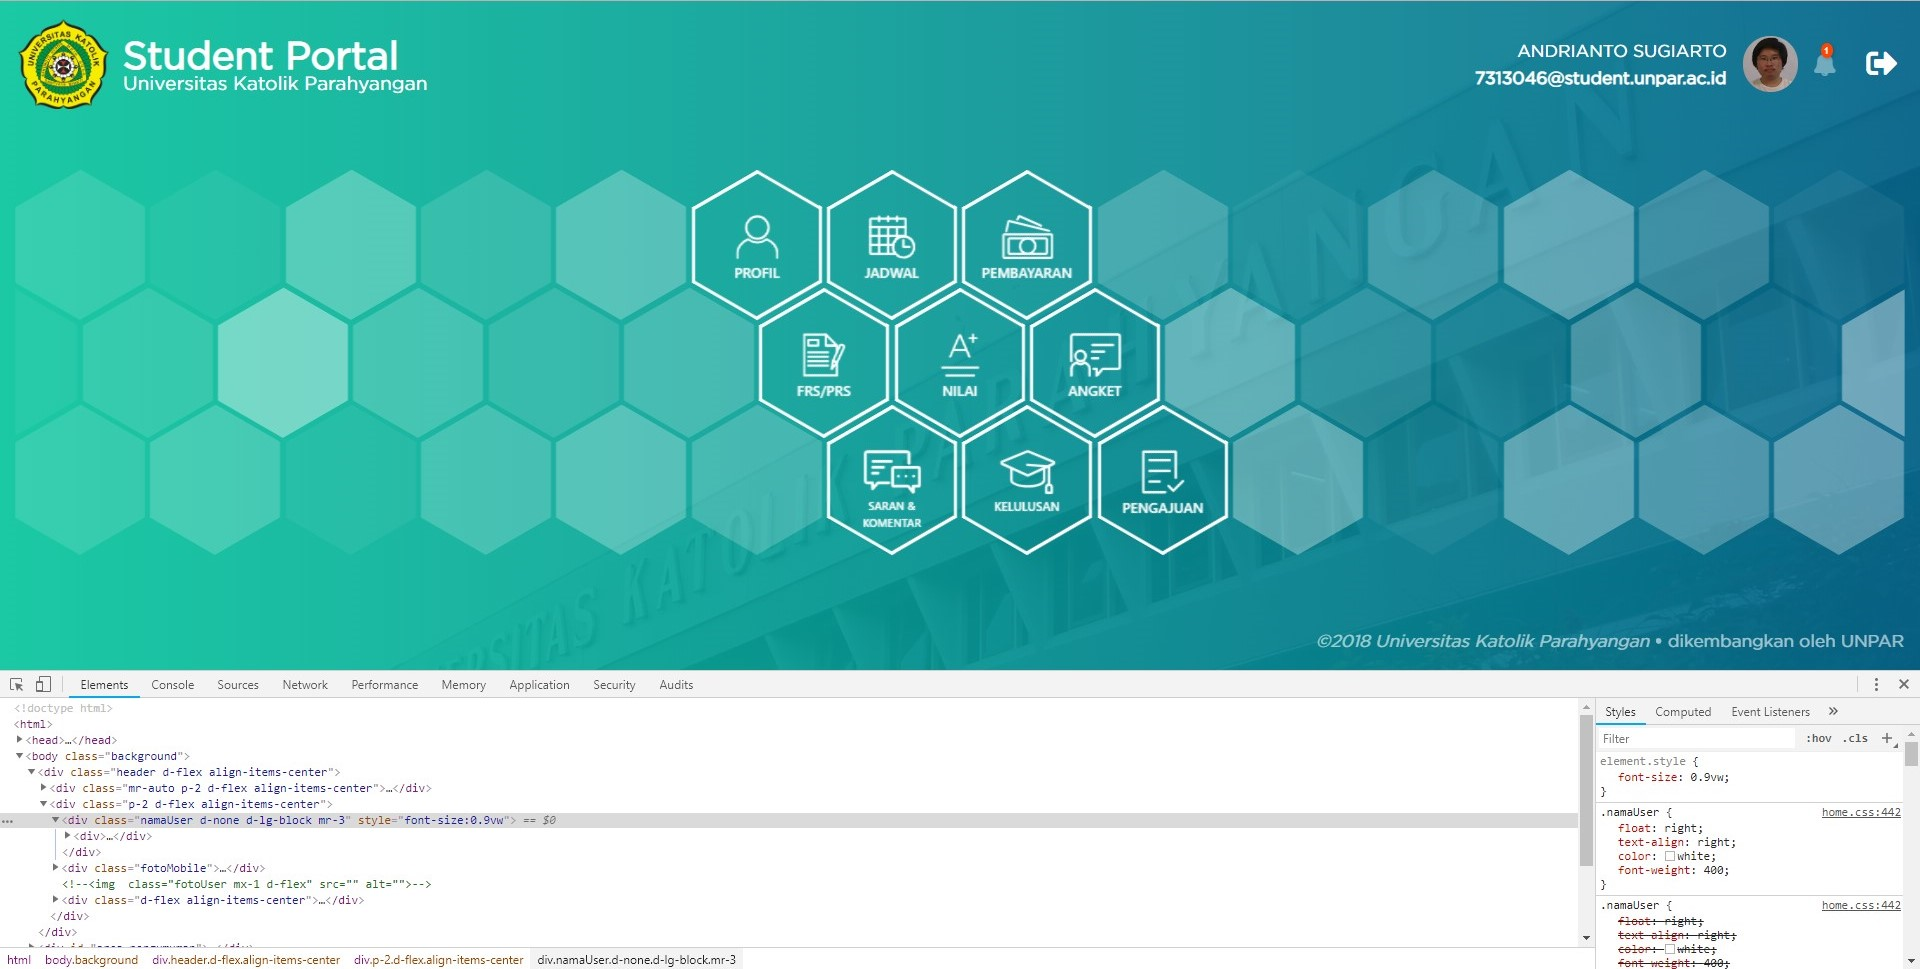
\includegraphics[scale=0.3]{Gambar/Home_nama_user}
			\caption{Elemen ``div.namaUser.d-none.d-lg-block.mr-3'' pada Halaman Home}
			\label{pic:home_nama_user}
		\end{figure}
		\begin{figure}[H]
			\centering
			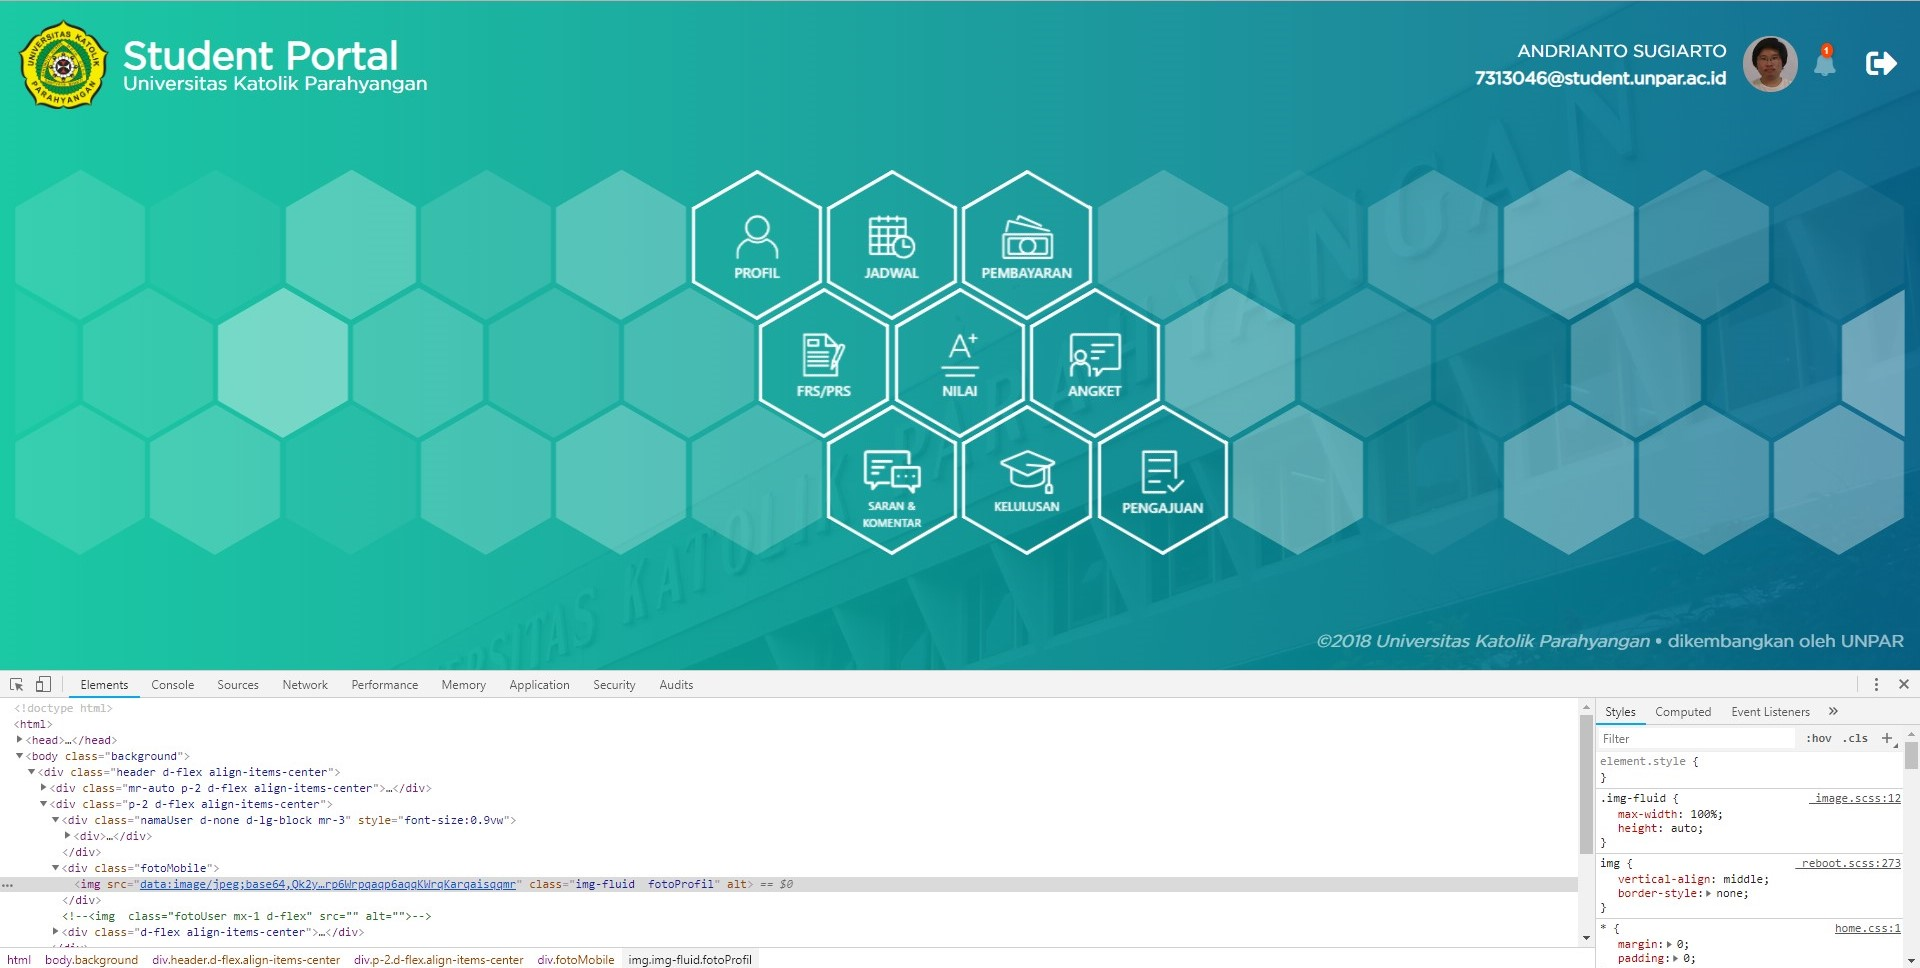
\includegraphics[scale=0.3]{Gambar/Home_foto_user}
			\caption{Elemen ``img.img-fluid.fotoProfil'' pada Halaman Home}
			\label{pic:home_foto_user}
		\end{figure}
Pada halaman ini terdapat data mahasiswa berupa nama dan foto mahasiswa yang didapatkan setelah login ke student portal. Data nama dan foto mahasiswa diproses menggunakan \textit{method} yang terdapat pada kelas \texttt{Scraper}, yaitu  \textit{method} \texttt{TahunSemester requestNamePhotoTahunSemester(String phpsessid, Mahasiswa mhs)}. Untuk memproses data nama dan foto mahasiswa dilakukan dengan cara:
\begin{enumerate}
	\item Melakukan koneksi ke \url{https://studentportal.unpar.ac.id/home}
	\item Setelah berhasil, mengambil data nama mahasiswa dengan melakukan kueri css menggunakan kueri ``div.namaUser.d-none.d-lg-block.mr-3'' (Gambar \ref{pic:home_nama_user})
	\item Setelah berhasil melakukan kueri css, akan mendapatkan nama dan email mahasiswa. Data yang dibutuhkan hanya nama mahasiswa, sehingga perlu memotong hasil kueri dari karakter pertama sampai indeks awal email mahasiswa. 
	\item Kemudian disimpan pada atribut kelas \texttt{Mahasiswa} dengan menggunakan \textit{method} \texttt{void setNama(String nama)}.
	\item Setelah berhasil menyimpan nama mahasiswa, kemudian melakukan kueri css untuk menyimpan foto mahasiswa menggunakan kueri ``img.img-fluid.fotoProfil'' (Gambar \ref{pic:home_foto_user})
	\item Setelah berhasil melakukan kueri css, akan mendapatkan foto mahasiswa dalam format \textit{Base64}. Disini perlu melakukan perubahan pada kelas \texttt{Mahasiswa}, yaitu:
	\begin{itemize}
		\item Atribut \texttt{URL photoUrl} menjadi \texttt{String photoPath}, karena data foto mahasiswa dalam format \textit{Base64}.
		\item \textit{Method} \texttt{URL getPhotoURL()} menjadi \texttt{String getPhotoPath()}, karena perubahan pada atribut dibutuhkan perubahan \textit{method getter}.
		\item \textit{Method} \texttt{void setPhotoURL(URL photoURL)} menjadi \texttt{void setPhotoPath(String photoPath)}, karena perubahan pada atribut dibutuhkan perubahan \textit{method setter}.
	\end{itemize}
	\item Kemudian disimpan pada atribut kelas \texttt{Mahasiswa} dengan menggunakan \textit{method} \texttt{void setPhotoPath(String photoPath)}
	\item Proses berikutnya akan dijelaskan pada sub sub-bab halaman FRS/PRS
\end{enumerate}

\subsection{Halaman FRS/PRS}
		\begin{figure}[H]
			\centering
			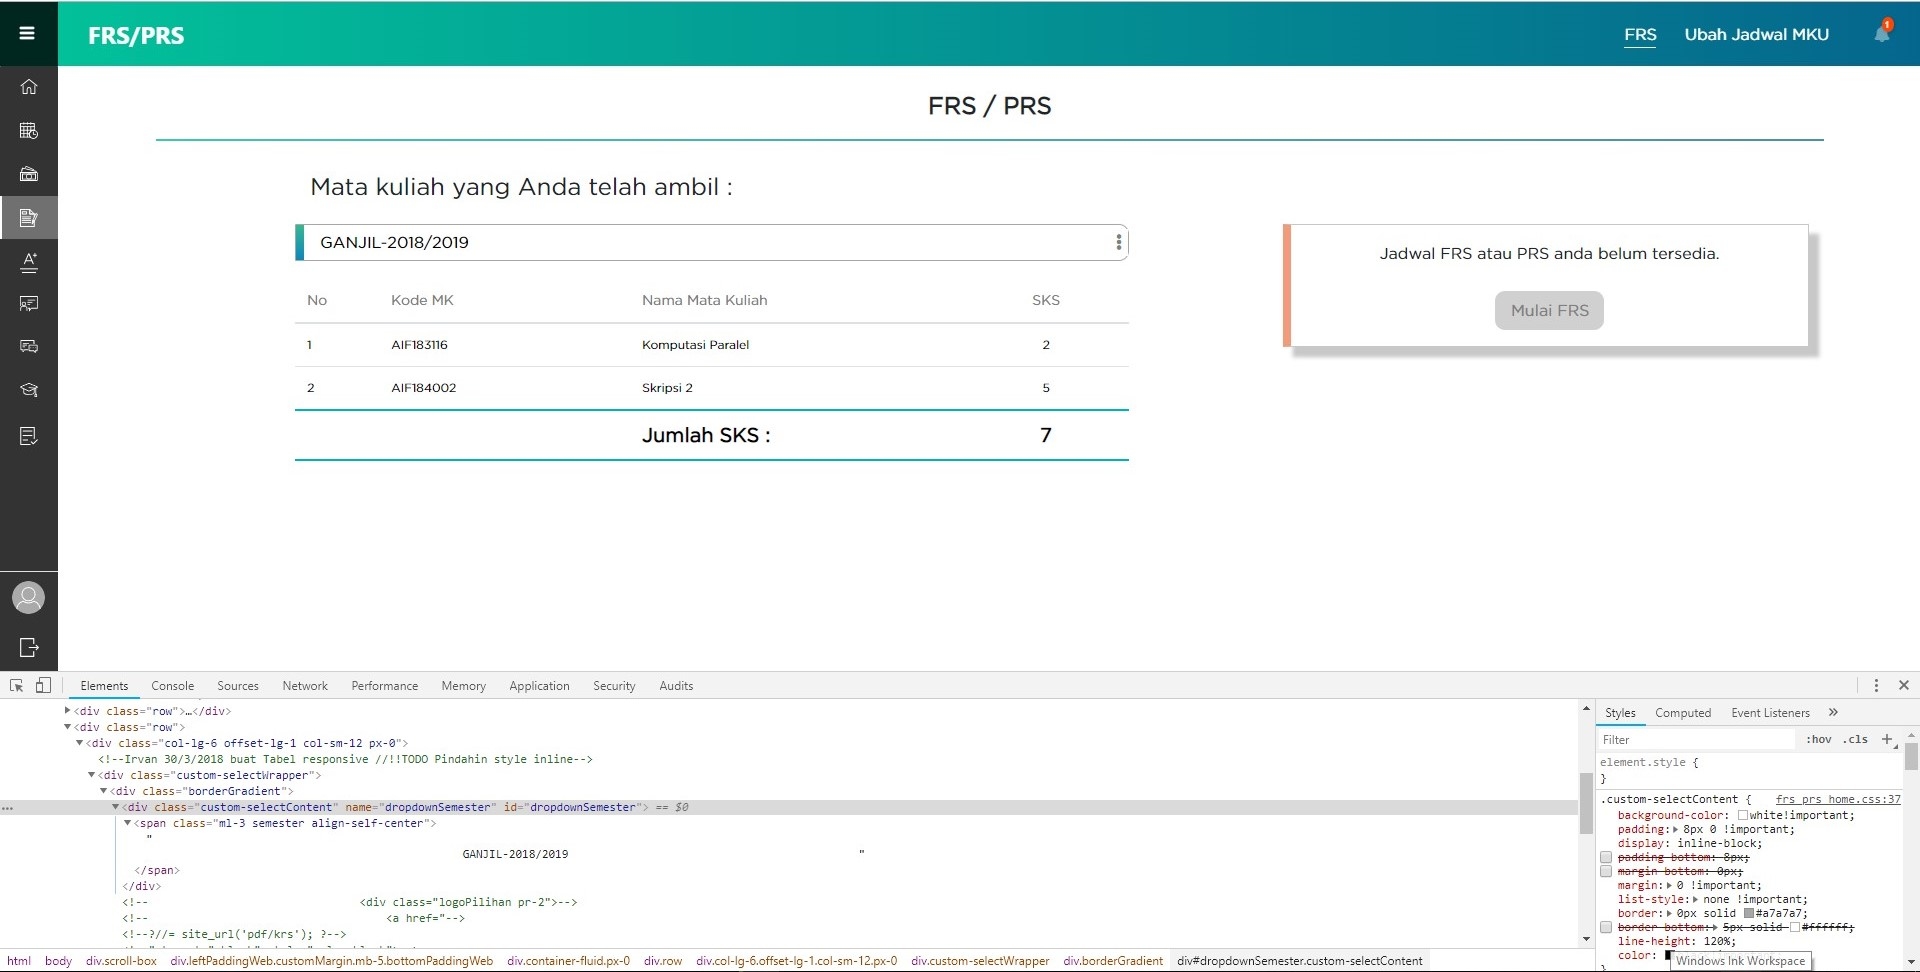
\includegraphics[scale=0.3]{Gambar/Home_semester_user}
			\caption{Elemen ``.custom-selectContent span'' pada Halaman FRS/PRS}
			\label{pic:home_semester_user}
		\end{figure}
Pada halaman ini terdapat data mahasiswa berupa tahun semester yang ditempuh oleh mahasiswa. Karena pada halaman home tidak bisa mendapatkan tahun semester yang ditempuh oleh mahasiswa, sehingga data tahun semester diambil dari halaman FRS/PRS. Data tahun semester diproses menggunakan \textit{method} yang terdapat pada kelas \texttt{Scraper}, yaitu  \textit{method} \texttt{TahunSemester requestNamePhotoTahunSemester(String phpsessid, Mahasiswa mhs)}. Untuk memproses data tahun semester dilakukan dengan cara:
\begin{enumerate}
	\item Melakukan koneksi ke \url{https://studentportal.unpar.ac.id/frs_prs}
	\item Setelah berhasil, mengambil data tahun semester mahasiswa dengan melakukan kueri css menggunakan kueri ``.custom-selectContent span'' (Gambar \ref{pic:home_semester_user})
	\item Setelah berhasil melakukan kueri css, akan didapatkan data tahun semester mahasiswa
	\item data tahun semester perlu diuraikan menjadi tahun dan semester yang disimpan pada \textit{array} tipe data \textit{String}, sehingga bisa disimpan pada atribut kelas \texttt{TahunSemester} dengan constructor \texttt{TahunSemester(int tahun, Semester semester)}
\end{enumerate}

\subsection{Halaman Jadwal}
		\begin{figure}[H]
			\centering
			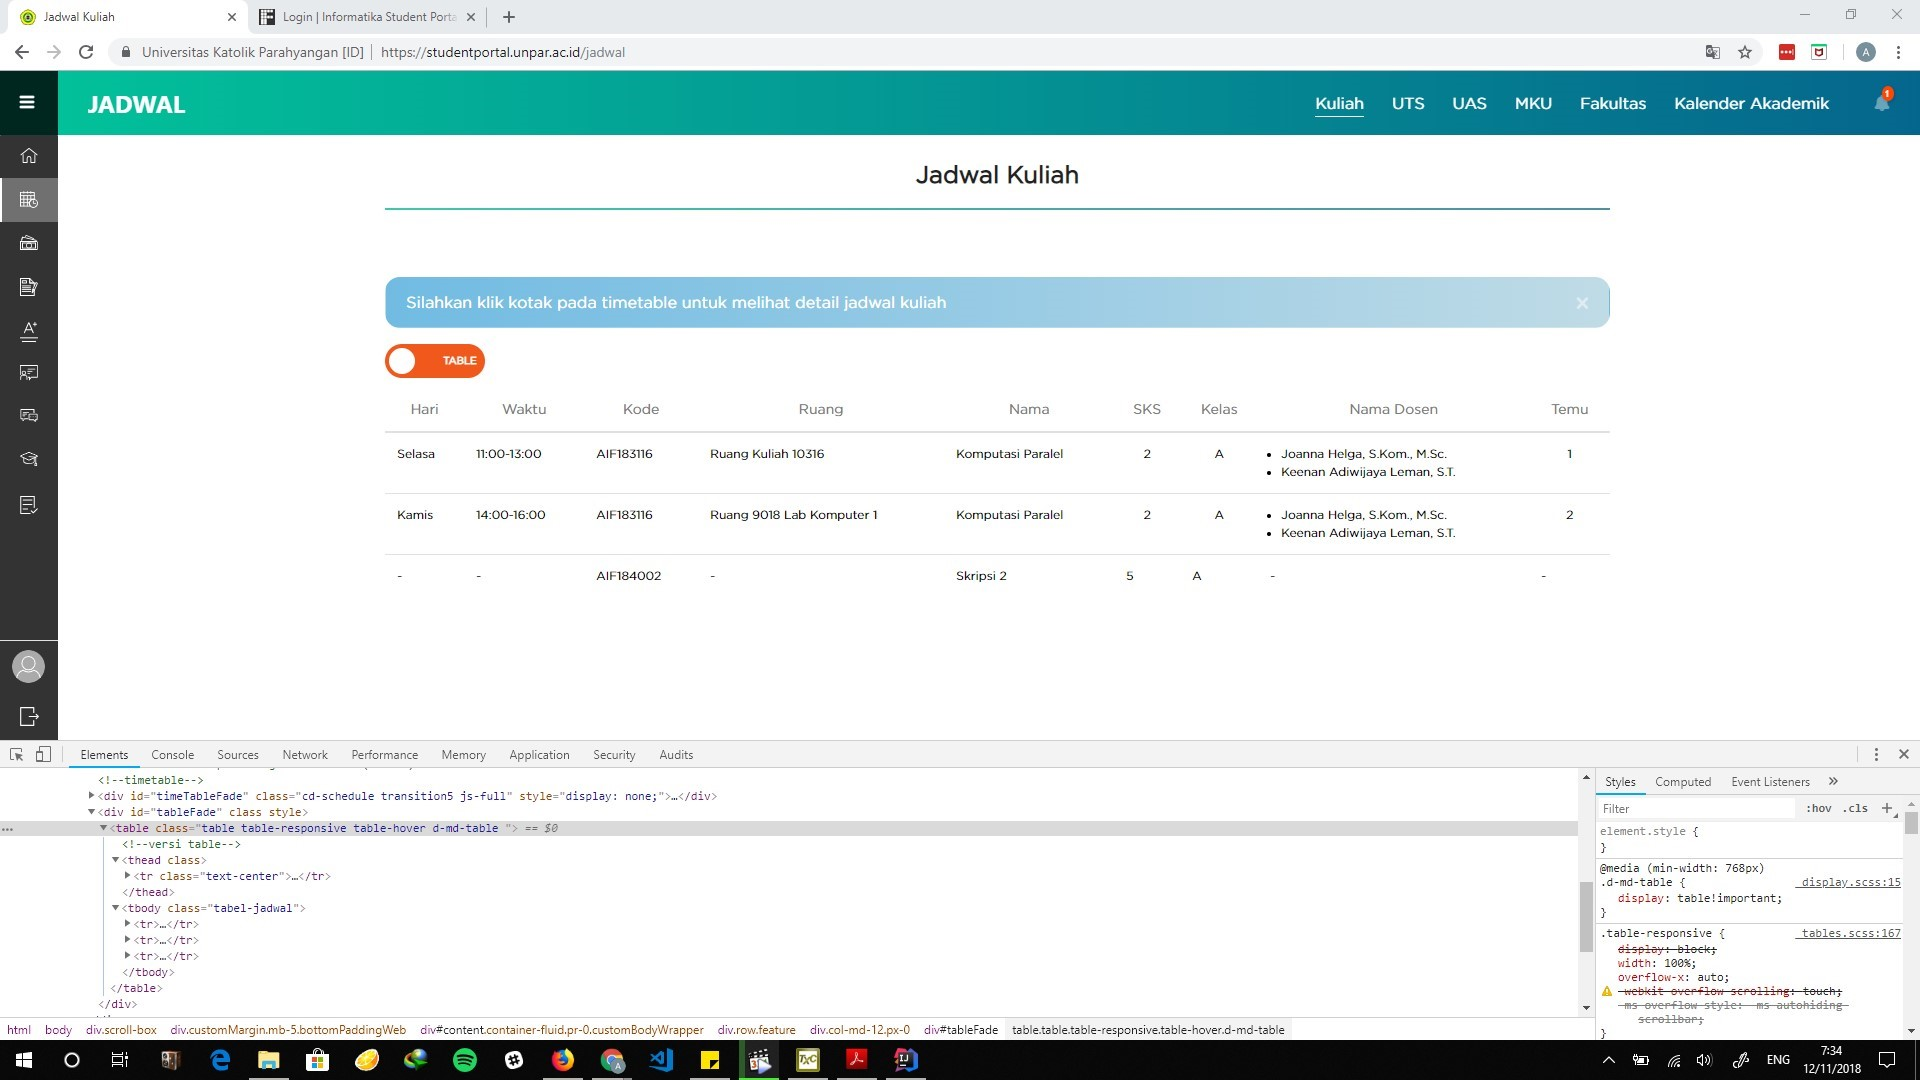
\includegraphics[scale=0.3]{Gambar/Jadwal_user}
			\caption{Elemen ``table.table.table-responsive.table-hover.d-md-table'' pada Halaman Jadwal}
			\label{pic:jadwal_user}
		\end{figure}
Pada halaman ini terdapat data jadwal kuliah dari mahasiswa. Data jadwal kuliah yang dibutuhkan untuk fitur jadwal kuliah pada IFStudentPortal diambil dari tampilan jadwal dalam bentuk tabel. Data jadwal kuliah diproses menggunakan \textit{method} yang terdapat pada kelas \texttt{Scraper}, yaitu  \textit{method} \texttt{List<JadwalKuliah> requestJadwal(String phpsessid)}. Untuk memproses data jadwal kuliah dilakukan dengan cara:
\begin{enumerate}
	\item Melakukan koneksi ke \url{https://studentportal.unpar.ac.id/jadwal}
	\item Setelah berhasil, mengambil data jadwal kuliah dengan melakukan kueri css menggunakan kueri ``table.table.table-responsive.table-hover.d-md-table'' (Gambar \ref{pic:jadwal_user}).
	\item Setelah berhasil melakukan kueri css, jika terdapat jadwal kuliah, maka jadwal kuliah diolah dan kemudian disimpan dalam sebuah daftar jadwal kuliah yang kemudian akan dikembalikan dalam bentuk daftar jadwal kuliah. 
\end{enumerate}

\subsection{Halaman Nilai}
		\begin{figure}[H]
			\centering
			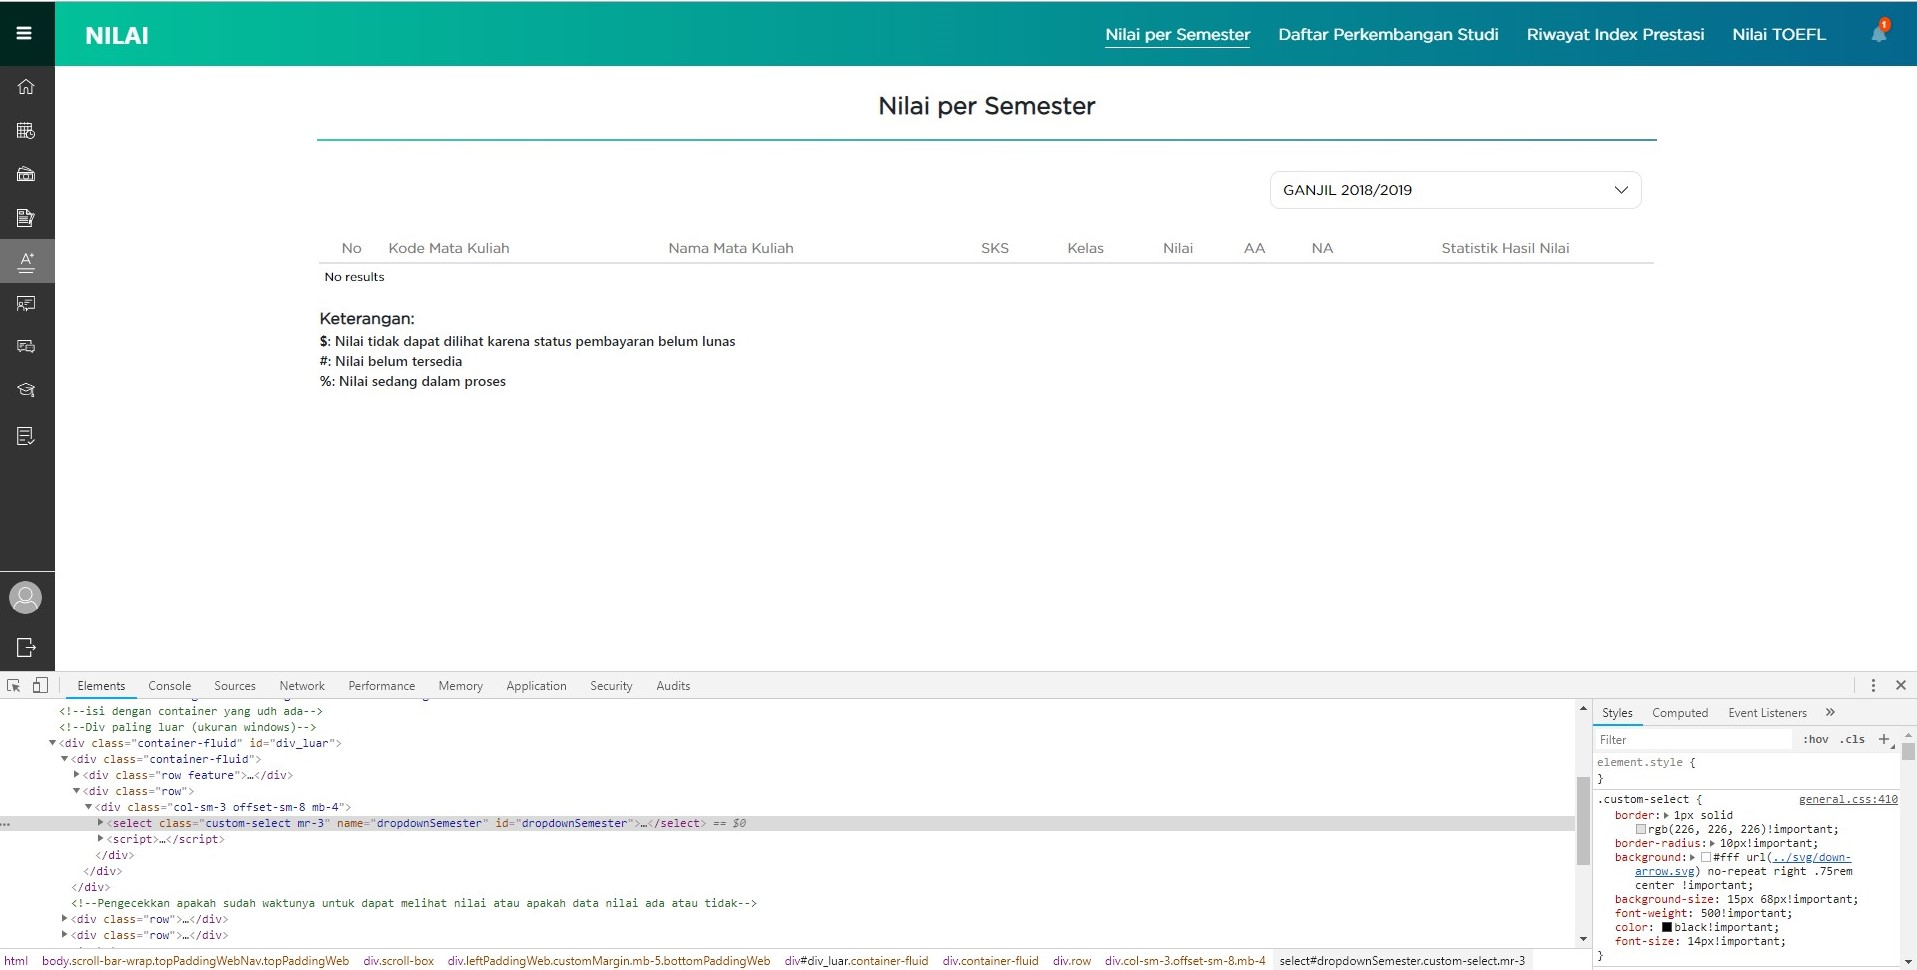
\includegraphics[scale=0.3]{Gambar/Nilai_combobox_user}
			\caption{\textit{Combo Box} ``select\#dropdownSemester.custom-select.mr-3'' pada Halaman Nilai}
			\label{pic:nilai_combobox_user}
		\end{figure}
Pada halaman ini terdapat data nilai mahasiswa terkini. Nilai yang diambil adalah nilai per semester yang sudah memuat kode mata kuliah yang berlaku di kurikulum 2018. Data nilai akan diproses menggunakan \textit{method} pada kelas \texttt{Scraper}, yaitu \textit{method} \texttt{void requestNilai(String phpsessid, Mahasiswa logged\_mhs)}. Untuk memproses daata nilai dilakukan dengan cara:
\begin{enumerate}
	\item Melakukan koneksi ke \url{https://studentportal.unpar.ac.id/nilai}
	\item Setelah berhasil, mengambil data nilai berdasarkan tahun dan semester dengan melakukan kueri css menggunakan kueri ``select\#dropdownSemester.custom-select.mr-3'' (Gambar \ref{pic:nilai_combobox_user})
	\item Setelah berhasil melakukan kueri css, kemudian disimpan pada atribut lokal \texttt{ArrayList<String> listSemester} dari atribut \textit{value} ``\textit{option}''
	\item Setelah berhasil menyimpan \textit{value ``option''} dari \textit{Combo Box}. Kemudian diperlukan melakukan koneksi berkali-kali sebanyak semester yang telah ditempuh mahasiswa, sehingga dibutuhkan waktu yang tidak sebentar. Karena pada halaman nilai tidak dapat menampilkan seluruh semester seperti Student Portal yang lama, sehingga untuk mengatasi masalah ini dibuat menjadi paralel. Untuk itu dibuat kelas yang mengimplementasikan kelas \textit{interface} \texttt{Runnable}, yaitu:
	\begin{itemize}
		\item \texttt{MultipleRequest}
		\begin{figure}[H]
			\centering
			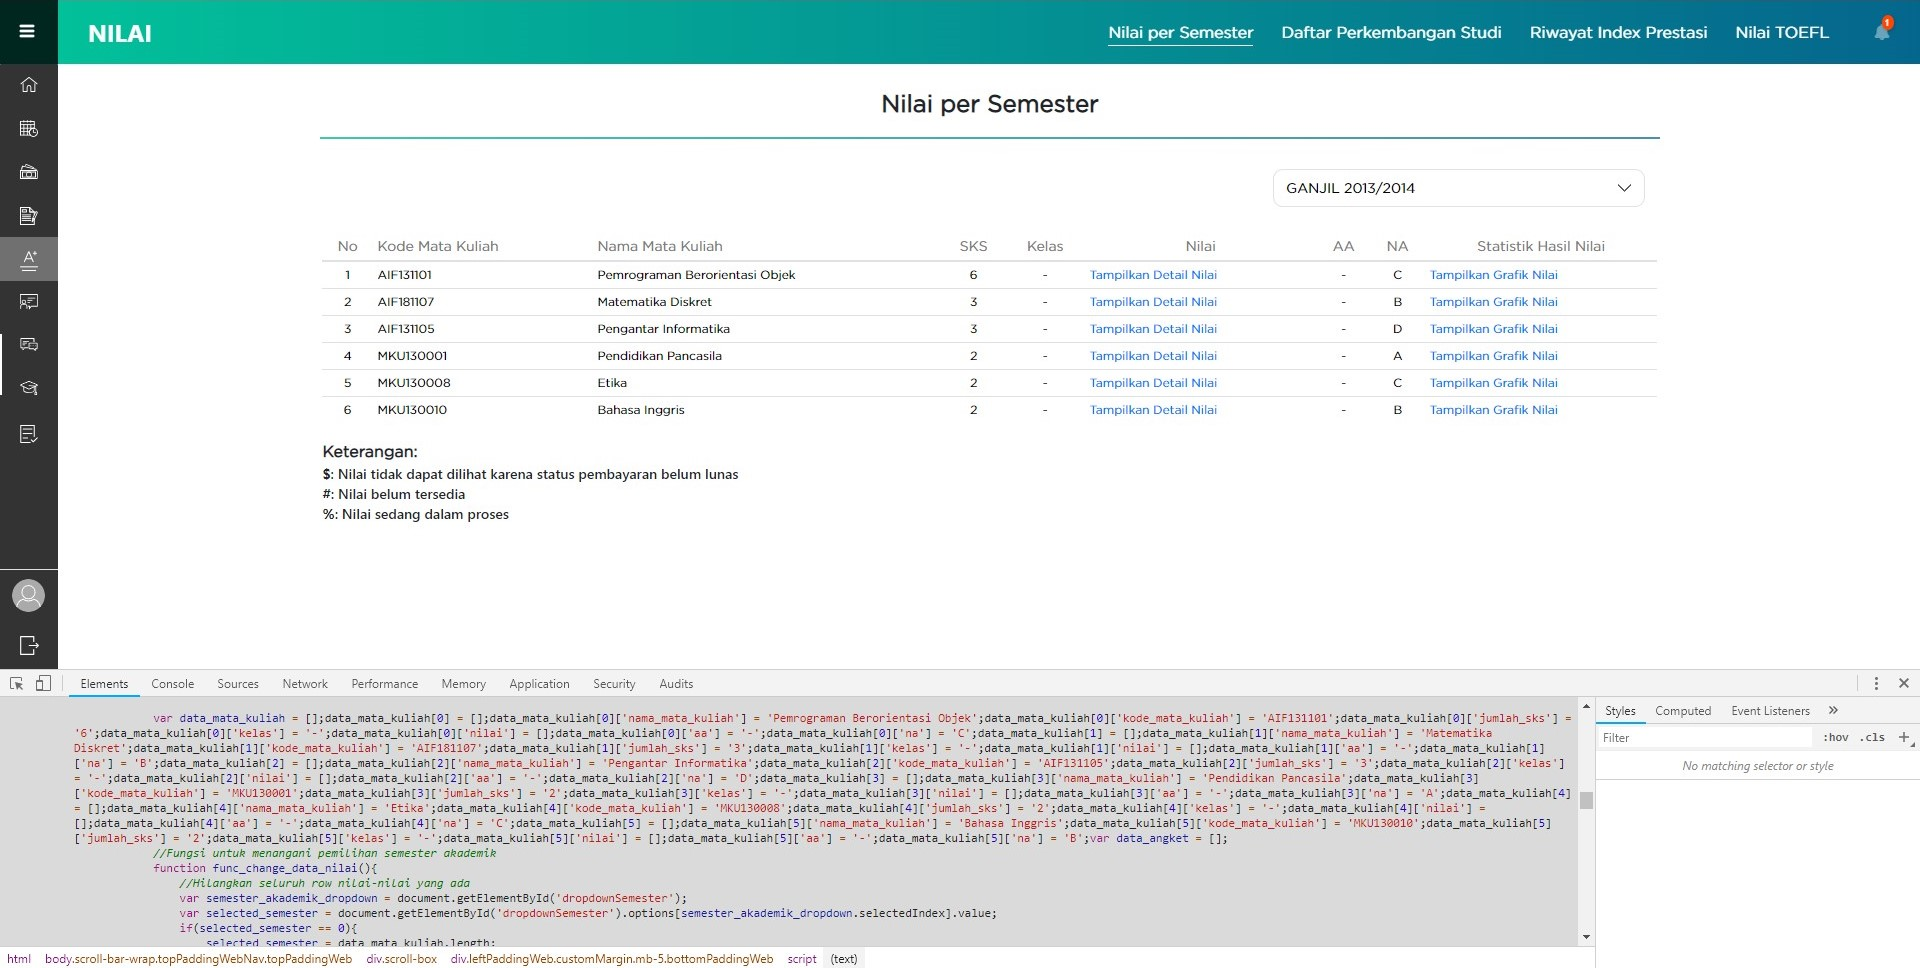
\includegraphics[scale=0.3]{Gambar/Nilai_per_semester_salah_satu}
			\caption{Script Data Nilai Mahasiswa Pada Halaman Nilai}
			\label{pic:nilai_per_semester_script}
		\end{figure}
		Pada kelas ini juga mengatasi masalah pengambilan data nilai dimana nilai di isi ke dalam tabel menggunakan \textit{javascript}. Atribut pada kelas ini merupakan atribut yang diperlukan untuk mendapatkan nilai mahasiswa, yaitu:
		\begin{itemize}
			\item Atribut \texttt{int l} merupakan atribut untuk menyimpan satu angka urutan dari atribut \texttt{listSemester}.
			\item Atribut \texttt{ArrayList<String> listSemester} merupakan daftar semester yang telah ditempuh mahasiswa.
			\item Atribut \texttt{String NILAI\_URL} merupakan alamat untuk mendapatkan nilai mahasiswa.
			\item Atribut \texttt{String phpsessid} untuk menyimpan \textit{cookies} dari \textit{login} ke Student Portal.
			\item Atribut \texttt{Mahasiswa logged\_mhs} untuk menyimpan data mahasiswa.
			\item Atribut \texttt{ScriptEngineManager factory} untuk menjalankan \textit{javascript}.
			\item Atribut \texttt{ScriptEngine engine} untuk menjalankan \textit{javascript}.
		\end{itemize}
		\textit{Method} yang dimiliki kelas ini adalah \texttt{void run}. \textit{Method} ini merupakan \textit{method} turunan dari kelas \texttt{interface Runnable}. Untuk mendapatkan data nilai dilakukan dengan cara:
		\begin{enumerate}
			\item Mendapatkan tahun dan semester yang ditempuh mahasiswa dari atribut \texttt{Arraylist<String> listSemester} diambil dari value atribut \texttt{int l}. Kemudian String dibagi menjadi tahun dan semester yang dibutuhkan.
			\item Setelah mendapatkan tahun dan semester. Kemudian melakukan koneksi ke alamat nilai berdasarkan tahun dan semester (\url{https://studentportal.unpar.ac.id/nilai/2013/1}).
			\item Setelah berhasil, kemudian melakukan kueri css berdasarkan script yang mengandung nilai mahasiswa (Gambar \ref{pic:nilai_per_semester_script}). 
			\item Selanjutnya adalah mendapatkan script yang mengandung script ``var data\_mata\_kuliah = [];'' sampai indeks dari ``var data\_angket = [];''.
			\item Setelah mendapatkan script yang dibutuhkan, selanjutnya menjalankan script menggunakan \textit{method} milik kelas \texttt{ScriptEngine} yaitu \texttt{Object eval(String script)}.
			\item Setelah berhasil, data yang didapatkan bertipe \texttt{ScriptObjectMirror} yang membungkus hasil eksekusi. Data nilai didapatkan dengan menggunakan \textit{method} \texttt{Object get(Object key)}.
			\item Setelah berhasil, kemudian memasukan data nilai ke daftar riwayat nilai mahasiswa pada atribut kelas \texttt{Mahasiswa} yaitu \texttt{List<Nilai> riwayatNilai} menggunakan method \texttt{List<Nilai> getRiwayatNilai()}. Proses ini dilakukan berulang kali sebanyak jumlah mata kuliah per semesternya.
		\end{enumerate}
	\end{itemize}
	\item Setelah berhasil mendapatkan seluruh nilai, kemudian data diurutkan berdasarkan tahun semester mata kuliah tersebut ditempuh.
\end{enumerate}

\subsection{Halaman Nilai TOEFL}
		\begin{figure}[H]
			\centering
			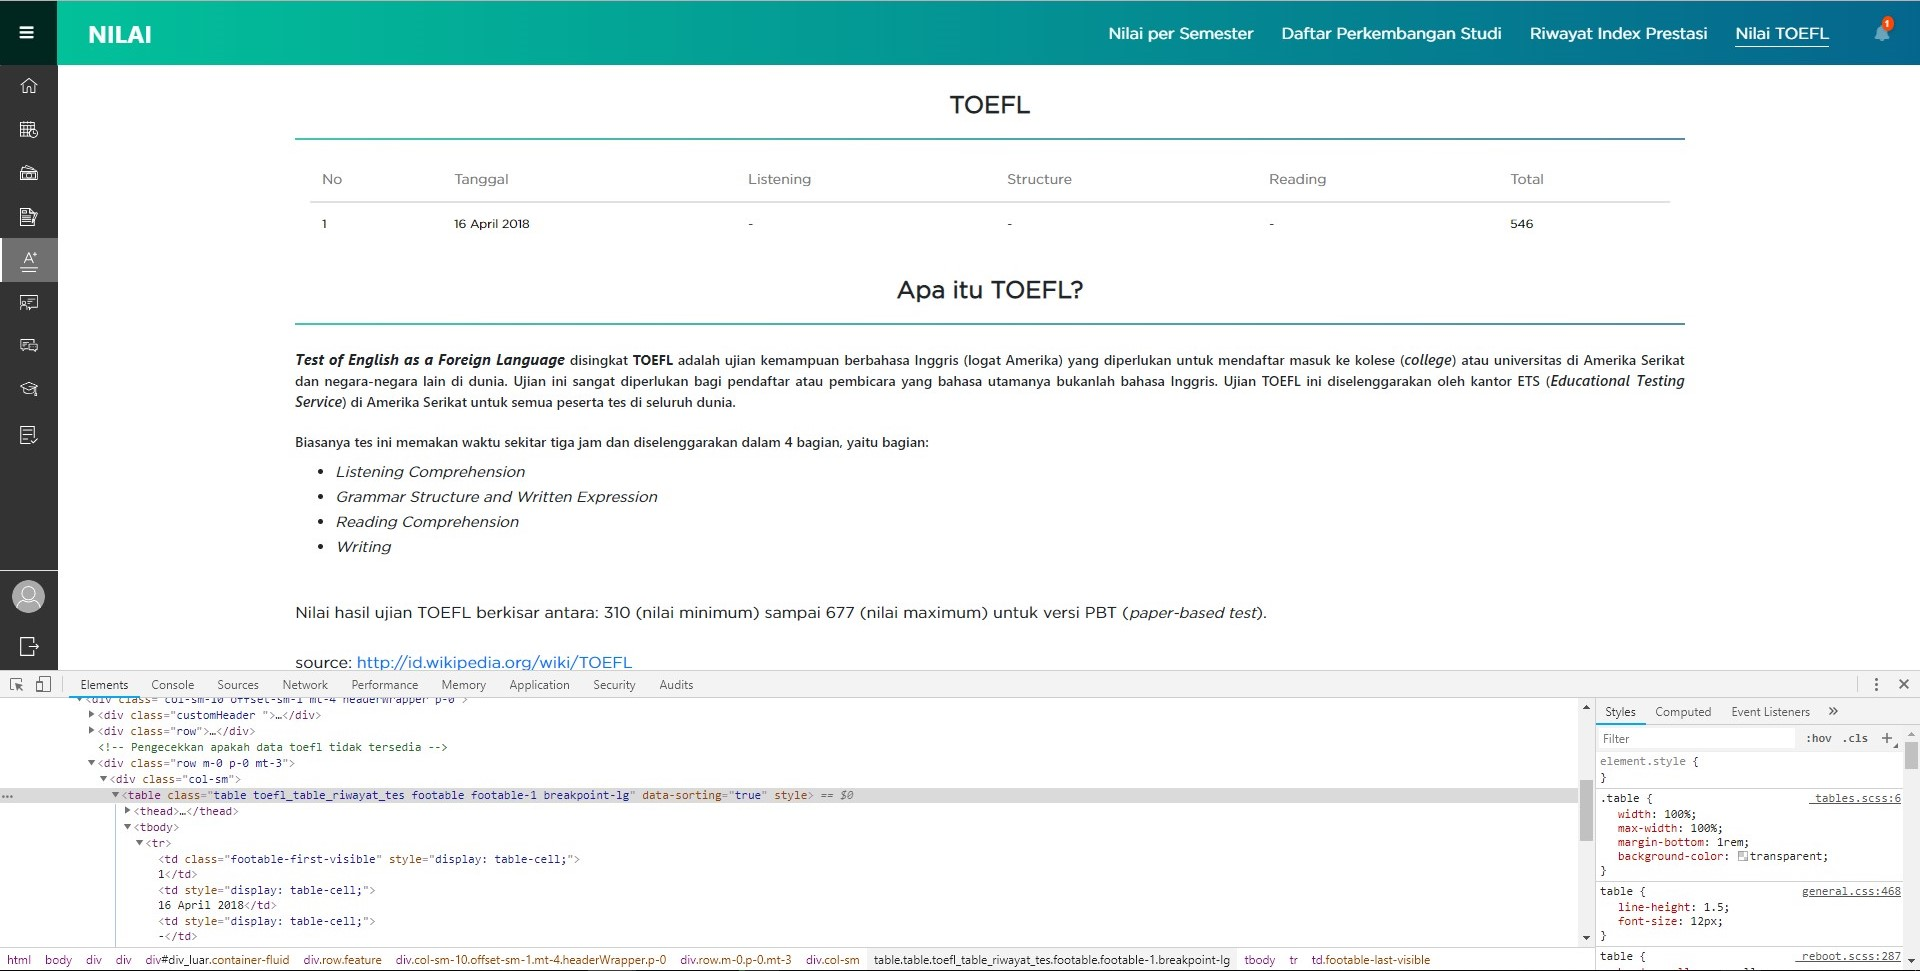
\includegraphics[scale=0.3]{Gambar/Nilai_toefl_css}
			\caption{Elemen ``table tbody tr'' dengan nilai TOEFL Mahasiswa}
			\label{pic:nilai_toefl_css}
		\end{figure}
Pada halaman ini terdapat data nilai TOEFL yang telah ditempuh oleh mahasiswa. Data nilai TOEFL akan diproses menggunakan \textit{method} pada kelas \texttt{Scraper}, yaitu \textit{method} \texttt{void requestNilaiTOEFL(String phpsessid, Mahasiswa mahasiswa)}. Untuk memproses data nilai TOEFL dilakukan dengan cara:
\begin{enumerate}
	\item Melakukan koneksi ke \url{https://studentportal.unpar.ac.id/nilai/toefl}
	\item Setelah berhasil, mengambil data nilai TOEFL dengan melakukan kueri css menggunakan kueri ``table'', ``tbody'', dan ``tr'' (Gambar \ref{pic:nilai_toefl_css})
	\item Setelah berhasil melakukan kueri css, akan mendapatkan data nilai TOEFL yang perlu diolah kemudian disimpan pada atribut kelas \textit{Mahasiswa} dengan menggunakan \textit{method} \texttt{void setNilaiTOEFL(SortedMap<LocalDate, Integer> nilaiTOEFL)}
\end{enumerate}

\section{Perancangan Antarmuka}
Pada antarmuka untuk IFStudentPortal tidak ada perubahan.